\documentclass[titlepage]{article}
\usepackage[10pt]{extsizes} 
\usepackage[T2A]{fontenc}
\usepackage[utf8]{inputenc}
\usepackage[english,russian]{babel}
%\usepackage{pscyr}
\usepackage{hyperref}
\usepackage{setspace}
\usepackage{amsmath,amssymb,amsfonts,amsthm,secdot}
\usepackage[left=30mm, top=20mm, right=30mm, bottom=20mm, nohead, footskip=15mm]{geometry} 
\usepackage[pdftex]{graphicx}
\usepackage[indentfirst]{titlesec}
\usepackage[usenames]{color}
\usepackage{colortbl}
\usepackage{listings}
\usepackage{secdot}

\def\l{\left}
\def\r{\right}
\def\le{\leqslant}
\def\ge{\geqslant}

\begin{document} 

\newtheorem{theorem}{Теорема}
\newtheorem{lemma}{Лемма}
\newtheorem{definition}{Определение}
\renewcommand{\proofname}{Доказательство}

\begin{center}
\hfill \break
\hfill \break
\hfill \break
\LARGE Приближенное решение задачи оптимального управления \\
\hfill \break
\large Михайлин Д.А. \\
\large 410 группа \\
\hfill \break
\today \\

\end{center}

\section{1. Постановка задачи}
Требуется найти приближенное задачи
\begin{gather*}
	\notag \int_{0}^{\frac{\pi}{2}}u^2dt \rightarrow inf \\
	\notag x(0) = 0; x(\frac{\pi}{2}) = 0; x'\l(\frac{\pi}{2}\r) = -\frac{\pi}{2}; \; x'' + xe^{-\alpha x} = 0; \; \alpha \in \left[0;25\right]\\
\end{gather*}

\section{2. Необходимые условия}
Сделаем замены:
\begin{gather*}
	\notag x_1 = x; \; x_2 = x_1'; \\
\end{gather*}

Тогда функция Лагранжа примет вид

\begin{gather*}
	\notag \mathcal{L} = \int_{0}^{\frac{\pi}{2}}\left[\lambda_0 u^2 + p_1 (x_1' - x_2) + p_2 (x_2' + x_1 e^{-\alpha x_1})\right] dt + \lambda_1 x_1(0) + \lambda_2 x_2(\frac{\pi}{2}) + \lambda_3(x_2(\frac{\pi}{2}) + \frac{\pi}{2}) \\
\end{gather*}

Из условий стационарности по $x_1$ и $x_2$ получим уравнения

\begin{gather*}
	\notag p_1' = -p_2 (-e^{-\alpha x_1} + \alpha x_1 e^{-\alpha x_1}) \\
	\notag p_2' = -p_1  \\
\end{gather*}

Из условий трансверсальности по $x_1$ и $x_2$ получим условия

\begin{gather*}
	\notag p_1(0) = \lambda_1;  p_2(0) = 0; \; p_1\l(\frac{\pi}{2}\r) = \lambda_2; \;  p_2\l(\frac{\pi}{2}\r) = \lambda_3; \\
\end{gather*}

Из условия оптимальности по $u$ получим $u = \frac{p_2}{2 \lambda_0}$, если $\lambda_0 \neq 0$. Если же $\lambda_0 = 0$, то из условий выше получаем, что либо минимум по $u$ не достигается, либо все
$\lambda_i = 0; p_i = 0$. Тогда положим $\lambda_0 = 1$, и тогда $u = \frac{p_2}{2}$.

\bigbreak
Получили систему из четырех уравнений с  начальными условиями

\bigbreak
$\begin{cases} 
	\notag x_1' = x_2\\
	\notag x_2' = p_2/2 - x_1 e^{-\alpha x_1}\\
	\notag p_1' = -p_2 (-e^{-\alpha x_1} + \alpha x_1 e^{-\alpha x_1}) \\
	\notag p_2' = -p_1 \\
	\notag x_1(0) = 0; \; p_2(0) = 0;
\end{cases} $
\bigbreak
и двумя условиями в правом конце

\begin{gather*}
	\notag x_1\l(\frac{\pi}{2}\r) = 0; \; x_2\l(\frac{\pi}{2}\r) = -\frac{\pi}{2}; \\
\end{gather*}

С помощью метода Ньютона будем искать решение $x_1(0)$ и $p_2(0)$ системы
\bigbreak
$
\begin{cases}
	\notag x_1\l(\frac{\pi}{2}\r) = 0 \\
	\notag x_2\l(\frac{\pi}{2}\r) + \frac{\pi}{2} = 0 \\
\end{cases}
$
\bigbreak
То есть будем искать недостающие левые условия так, чтобы попасть в правые.

\section{3. Аналитическое решение в случае $\alpha = 0$}

В этом случае система примет вид
\bigbreak
$\begin{cases} 
	\notag x_1' = x_2\\
	\notag x_2' = p_2/2 - x_1 e^{-\alpha x_1}\\
	\notag p_1' = -p_2 (-e^{-\alpha x_1} + \alpha x_1 e^{-\alpha x_1}) \\
	\notag p_2' = -p_1 \\
	\notag x_1(0) = 0; \; p_2(0) = 0;
	\notag x_1(\frac{\pi}{2}) = 0; \; x_2(\frac{\pi}{2}) = -\frac{\pi}{2};
\end{cases} $
\bigbreak

Вторые два уравнения дают нам:

\begin{gather*}
	\notag p_1 = c_1\sin{t} + c_4\cos{t}, \; p_2 = c_1\cos{t} - c_4\sin{t} \\
\end{gather*}

Первые два уравнения дают нам, с учетом двух последних уравнений:

\begin{gather*}
	\notag x_1(t) = \frac{1}{4}c_1t\sin{t} + c_3\sin{t} + c_2\cos{t} + \frac{1}{4}c_4(t\cos{t} - sin{t}) \\
	\notag x_2(t) = -c_2\sin{t} - \frac{1}{4}c_4t\sin{t} + c_3cos{t} + \frac{1}{4}c_1(\sin{t} + tcos{t})\\
\end{gather*}

Тогда, подставляя начальные условия получаем:

\begin{gather*}
	\notag p_2(t) = -4sin{t};
	\notag u = -2sin{t};
\end{gather*}

\begin{gather*}
	\notag \int_{0}^{\frac{\pi}{2}}u^2dt = 4\int_{0}^{\frac{\pi}{2}}\sin^2{t}dt = \pi \\	
\end{gather*}

Проверим достаточное условие на минимум, пусть $\widehat{x} + x$ - допустимая функция, тогда

\begin{gather*}
	\notag x'(\frac{\pi}{2}) = 0, \; x\l(\frac{\pi}{2}\r) = 0, x(0) = 0\\
	\notag \mathcal{F}(\widehat{x} + x) - \mathcal{F}(\widehat{x}) = \int_{0}^{\frac{\pi}{2}}\l[ (\widehat{x}'' + x'' + \widehat{x} + x)^2 - (\widehat{x}'' + \widehat{x})^2 \r]dt = \int_{0}^{\frac{\pi}{2}}\l[ 2(\widehat{x}'' + \widehat{x})(x'' + x) + (x'' + x)^2 \r]dt\\ = \int_{0}^{\frac{\pi}{2}}\l[ 2c\sin{t}(x'' + x) + (x'' + x)^2 \r]dt \\
\end{gather*}

При этом

\begin{gather*}
	\notag \int_{0}^{\frac{\pi}{2}} cx''\sin{t} dt = \int_{0}^{\frac{\pi}{2}} c\sin{t} dx' = cx'\sin{t}\vert_0^{\frac{\pi}{2}} - \int_{0}^{\frac{\pi}{2}} cx'\cos{t} dt \\
	\notag = -\int_{0}^{\frac{\pi}{2}} c\cos{t} dx = -cx\sin{t}\vert_0^{\frac{\pi}{2}} - \int_{0}^{\frac{\pi}{2}} cx\sin{t} dt = - \int_{0}^{\frac{\pi}{2}} cx\sin{t} dt \\	
\end{gather*}

Следовательно

\begin{gather*}
	\notag \mathcal{F}(\widehat{x} + x) - \mathcal{F}(\widehat{x}) = \int_{0}^{\frac{\pi}{2}}(x'' + x)^2 dt\geq 0\\	
\end{gather*}

Следовательно найденные функции доставляют глобальный минимум задачи.


\section{4. Результаты}

Будем запускать метод Ньютона в точках сетки $i=\overline{-10,10}, \; j=\overline{-10,10}$.

\subsection{$\alpha = 0.000000$} 
Метод Ньютона сошелся с большого количества начальных точек к результатам, указанным ниже. \\ 
\begin{tabular}{ | c | c | c | c |} 
\hline 
Initial point  & Newton method result & Right point & Functional 
 \\ $x_2(0), \; p_1(0)$ & $x_2(0), \; p_1(0)$ & $x_1\l(\frac{\pi}{2}\r), \; x_2\l(\frac{\pi}{2}\r)$ & $\int_{0}^{\frac{\pi}{2}}u^2dt$  \\ \hline 
0.000000e+00; 0.000000e+00 & 1.000000e+00; 4.000000e+00 & 4.260481e-14; -1.570796e+00 & 3.141593e+00 \\ \hline 
1.000000e+00; -1.000000e+00 & 1.000000e+00; 4.000000e+00 & 5.820344e-14; -1.570796e+00 & 3.141593e+00 \\ \hline 
2.000000e+00; -2.000000e+00 & 1.000000e+00; 4.000000e+00 & 4.428402e-14; -1.570796e+00 & 3.141593e+00 \\ \hline 
3.000000e+00; -3.000000e+00 & 1.000000e+00; 4.000000e+00 & 4.965472e-14; -1.570796e+00 & 3.141593e+00 \\ \hline 
4.000000e+00; -4.000000e+00 & 1.000000e+00; 4.000000e+00 & 4.284073e-14; -1.570796e+00 & 3.141593e+00 \\ \hline 
5.000000e+00; -5.000000e+00 & 1.000000e+00; 4.000000e+00 & 4.395095e-14; -1.570796e+00 & 3.141593e+00 \\ \hline 
6.000000e+00; -6.000000e+00 & 1.000000e+00; 4.000000e+00 & 4.256318e-14; -1.570796e+00 & 3.141593e+00 \\ \hline 
7.000000e+00; -7.000000e+00 & 1.000000e+00; 4.000000e+00 & 4.243828e-14; -1.570796e+00 & 3.141593e+00 \\ \hline 
\end{tabular} 
\subsection{$\alpha = 0.500000$} 
Метод Ньютона сошелся с большого количества начальных точек к результатам, указанным ниже. \\ 
\begin{tabular}{ | c | c | c | c |} 
\hline 
Initial point  & Newton method result & Right point & Functional 
 \\ $x_2(0), \; p_1(0)$ & $x_2(0), \; p_1(0)$ & $x_1\l(\frac{\pi}{2}\r), \; x_2\l(\frac{\pi}{2}\r)$ & $\int_{0}^{\frac{\pi}{2}}u^2dt$  \\ \hline 
0.000000e+00; 0.000000e+00 & 9.369253e-01; 3.843168e+00 & -1.061651e-14; -1.570796e+00 & 3.449121e+00 \\ \hline 
1.000000e+00; -1.000000e+00 & 9.369253e-01; 3.843168e+00 & -3.996803e-15; -1.570796e+00 & 3.449121e+00 \\ \hline 
2.000000e+00; -2.000000e+00 & 9.369253e-01; 3.843168e+00 & -4.933554e-15; -1.570796e+00 & 3.449121e+00 \\ \hline 
3.000000e+00; -3.000000e+00 & 9.369253e-01; 3.843168e+00 & -7.049916e-15; -1.570796e+00 & 3.449121e+00 \\ \hline 
4.000000e+00; -4.000000e+00 & 9.369253e-01; 3.843168e+00 & -1.543210e-14; -1.570796e+00 & 3.449121e+00 \\ \hline 
5.000000e+00; -5.000000e+00 & 9.369253e-01; 3.843168e+00 & -8.049117e-15; -1.570796e+00 & 3.449121e+00 \\ \hline 
6.000000e+00; -6.000000e+00 & 9.369253e-01; 3.843168e+00 & -6.161738e-15; -1.570796e+00 & 3.449121e+00 \\ \hline 
7.000000e+00; -7.000000e+00 & 9.369253e-01; 3.843168e+00 & -5.995204e-15; -1.570796e+00 & 3.449121e+00 \\ \hline 
\end{tabular} 
\subsection{$\alpha = 1.000000$} 
Метод Ньютона сошелся с большого количества начальных точек к результатам, указанным ниже. \\ 
\begin{tabular}{ | c | c | c | c |} 
\hline 
Initial point  & Newton method result & Right point & Functional 
 \\ $x_2(0), \; p_1(0)$ & $x_2(0), \; p_1(0)$ & $x_1\l(\frac{\pi}{2}\r), \; x_2\l(\frac{\pi}{2}\r)$ & $\int_{0}^{\frac{\pi}{2}}u^2dt$  \\ \hline 
0.000000e+00; 0.000000e+00 & 8.956807e-01; 3.747988e+00 & -1.866216e-14; -1.570796e+00 & 3.680434e+00 \\ \hline 
1.000000e+00; -1.000000e+00 & 8.956807e-01; 3.747988e+00 & -2.096934e-14; -1.570796e+00 & 3.680434e+00 \\ \hline 
2.000000e+00; -2.000000e+00 & 8.956807e-01; 3.747988e+00 & -2.395306e-14; -1.570796e+00 & 3.680434e+00 \\ \hline 
3.000000e+00; -3.000000e+00 & 8.956807e-01; 3.747988e+00 & -2.436940e-14; -1.570796e+00 & 3.680434e+00 \\ \hline 
4.000000e+00; -4.000000e+00 & 8.956807e-01; 3.747988e+00 & -1.968564e-14; -1.570796e+00 & 3.680434e+00 \\ \hline 
5.000000e+00; -5.000000e+00 & 8.956807e-01; 3.747988e+00 & -2.045239e-14; -1.570796e+00 & 3.680434e+00 \\ \hline 
6.000000e+00; -6.000000e+00 & 8.956807e-01; 3.747988e+00 & -2.240569e-14; -1.570796e+00 & 3.680434e+00 \\ \hline 
7.000000e+00; -7.000000e+00 & 8.956807e-01; 3.747988e+00 & -2.190956e-14; -1.570796e+00 & 3.680434e+00 \\ \hline 
\end{tabular} 
\subsection{$\alpha = 1.500000$} 
Метод Ньютона сошелся с большого количества начальных точек к результатам, указанным ниже. \\ 
\begin{tabular}{ | c | c | c | c |} 
\hline 
Initial point  & Newton method result & Right point & Functional 
 \\ $x_2(0), \; p_1(0)$ & $x_2(0), \; p_1(0)$ & $x_1\l(\frac{\pi}{2}\r), \; x_2\l(\frac{\pi}{2}\r)$ & $\int_{0}^{\frac{\pi}{2}}u^2dt$  \\ \hline 
0.000000e+00; 0.000000e+00 & 8.669897e-01; 3.688909e+00 & -2.281508e-14; -1.570796e+00 & 3.860734e+00 \\ \hline 
1.000000e+00; -1.000000e+00 & 8.669897e-01; 3.688909e+00 & -2.517431e-14; -1.570796e+00 & 3.860734e+00 \\ \hline 
2.000000e+00; -2.000000e+00 & 8.669897e-01; 3.688909e+00 & -2.083403e-14; -1.570796e+00 & 3.860734e+00 \\ \hline 
3.000000e+00; -3.000000e+00 & 8.669897e-01; 3.688909e+00 & -2.237793e-14; -1.570796e+00 & 3.860734e+00 \\ \hline 
4.000000e+00; -4.000000e+00 & 8.669897e-01; 3.688909e+00 & -2.570166e-14; -1.570796e+00 & 3.860734e+00 \\ \hline 
5.000000e+00; -5.000000e+00 & 8.669897e-01; 3.688909e+00 & -2.355754e-14; -1.570796e+00 & 3.860734e+00 \\ \hline 
6.000000e+00; -6.000000e+00 & 8.669897e-01; 3.688909e+00 & -4.387810e-14; -1.570796e+00 & 3.860734e+00 \\ \hline 
7.000000e+00; -7.000000e+00 & 8.669897e-01; 3.688909e+00 & -2.081321e-14; -1.570796e+00 & 3.860734e+00 \\ \hline 
\end{tabular} 
\subsection{$\alpha = 2.000000$} 
Метод Ньютона сошелся с большого количества начальных точек к результатам, указанным ниже. \\ 
\begin{tabular}{ | c | c | c | c |} 
\hline 
Initial point  & Newton method result & Right point & Functional 
 \\ $x_2(0), \; p_1(0)$ & $x_2(0), \; p_1(0)$ & $x_1\l(\frac{\pi}{2}\r), \; x_2\l(\frac{\pi}{2}\r)$ & $\int_{0}^{\frac{\pi}{2}}u^2dt$  \\ \hline 
0.000000e+00; 0.000000e+00 & 8.463221e-01; 3.652973e+00 & -1.897527e-14; -1.570796e+00 & 4.004377e+00 \\ \hline 
1.000000e+00; -1.000000e+00 & 8.463221e-01; 3.652973e+00 & -2.357142e-14; -1.570796e+00 & 4.004377e+00 \\ \hline 
2.000000e+00; -2.000000e+00 & 8.463221e-01; 3.652973e+00 & -1.966829e-14; -1.570796e+00 & 4.004377e+00 \\ \hline 
3.000000e+00; -3.000000e+00 & 8.463221e-01; 3.652973e+00 & -1.924849e-14; -1.570796e+00 & 4.004377e+00 \\ \hline 
4.000000e+00; -4.000000e+00 & 8.463221e-01; 3.652973e+00 & -2.137006e-14; -1.570796e+00 & 4.004377e+00 \\ \hline 
5.000000e+00; -5.000000e+00 & 8.463221e-01; 3.652973e+00 & -2.178336e-14; -1.570796e+00 & 4.004377e+00 \\ \hline 
6.000000e+00; -6.000000e+00 & 8.463221e-01; 3.652973e+00 & -2.047668e-14; -1.570796e+00 & 4.004377e+00 \\ \hline 
7.000000e+00; -7.000000e+00 & 8.463221e-01; 3.652973e+00 & -1.882348e-14; -1.570796e+00 & 4.004377e+00 \\ \hline 
\end{tabular} 
\subsection{$\alpha = 2.500000$} 
Метод Ньютона сошелся с большого количества начальных точек к результатам, указанным ниже. \\ 
\begin{tabular}{ | c | c | c | c |} 
\hline 
Initial point  & Newton method result & Right point & Functional 
 \\ $x_2(0), \; p_1(0)$ & $x_2(0), \; p_1(0)$ & $x_1\l(\frac{\pi}{2}\r), \; x_2\l(\frac{\pi}{2}\r)$ & $\int_{0}^{\frac{\pi}{2}}u^2dt$  \\ \hline 
0.000000e+00; 0.000000e+00 & 8.311276e-01; 3.632643e+00 & -1.381881e-14; -1.570796e+00 & 4.120476e+00 \\ \hline 
1.000000e+00; -1.000000e+00 & 8.311276e-01; 3.632643e+00 & -2.455067e-14; -1.570796e+00 & 4.120476e+00 \\ \hline 
2.000000e+00; -2.000000e+00 & 8.311276e-01; 3.632643e+00 & -1.760571e-14; -1.570796e+00 & 4.120476e+00 \\ \hline 
3.000000e+00; -3.000000e+00 & 8.311276e-01; 3.632643e+00 & -1.783990e-14; -1.570796e+00 & 4.120476e+00 \\ \hline 
4.000000e+00; -4.000000e+00 & 8.311276e-01; 3.632643e+00 & -1.693697e-14; -1.570796e+00 & 4.120476e+00 \\ \hline 
5.000000e+00; -5.000000e+00 & 8.311276e-01; 3.632643e+00 & -1.683115e-14; -1.570796e+00 & 4.120476e+00 \\ \hline 
6.000000e+00; -6.000000e+00 & 8.311276e-01; 3.632643e+00 & -1.699769e-14; -1.570796e+00 & 4.120476e+00 \\ \hline 
7.000000e+00; -7.000000e+00 & 8.311276e-01; 3.632643e+00 & -1.746346e-14; -1.570796e+00 & 4.120476e+00 \\ \hline 
\end{tabular} 
\subsection{$\alpha = 3.000000$} 
Метод Ньютона сошелся с большого количества начальных точек к результатам, указанным ниже. \\ 
\begin{tabular}{ | c | c | c | c |} 
\hline 
Initial point  & Newton method result & Right point & Functional 
 \\ $x_2(0), \; p_1(0)$ & $x_2(0), \; p_1(0)$ & $x_1\l(\frac{\pi}{2}\r), \; x_2\l(\frac{\pi}{2}\r)$ & $\int_{0}^{\frac{\pi}{2}}u^2dt$  \\ \hline 
0.000000e+00; 0.000000e+00 & 8.198264e-01; 3.623122e+00 & -1.181694e-14; -1.570796e+00 & 4.215244e+00 \\ \hline 
1.000000e+00; -1.000000e+00 & 8.198264e-01; 3.623122e+00 & 1.544945e-14; -1.570796e+00 & 4.215244e+00 \\ \hline 
2.000000e+00; -2.000000e+00 & 8.198264e-01; 3.623122e+00 & -2.877559e-14; -1.570796e+00 & 4.215244e+00 \\ \hline 
3.000000e+00; -3.000000e+00 & 8.198264e-01; 3.623122e+00 & -1.072406e-14; -1.570796e+00 & 4.215244e+00 \\ \hline 
4.000000e+00; -4.000000e+00 & 8.198264e-01; 3.623122e+00 & -1.375289e-14; -1.570796e+00 & 4.215244e+00 \\ \hline 
5.000000e+00; -5.000000e+00 & 8.198264e-01; 3.623122e+00 & -1.175102e-14; -1.570796e+00 & 4.215244e+00 \\ \hline 
6.000000e+00; -6.000000e+00 & 8.198264e-01; 3.623122e+00 & -1.337819e-14; -1.570796e+00 & 4.215244e+00 \\ \hline 
7.000000e+00; -7.000000e+00 & 8.198264e-01; 3.623122e+00 & -1.072406e-14; -1.570796e+00 & 4.215244e+00 \\ \hline 
\end{tabular} 
\subsection{$\alpha = 3.500000$} 
Метод Ньютона сошелся с большого количества начальных точек к результатам, указанным ниже. \\ 
\begin{tabular}{ | c | c | c | c |} 
\hline 
Initial point  & Newton method result & Right point & Functional 
 \\ $x_2(0), \; p_1(0)$ & $x_2(0), \; p_1(0)$ & $x_1\l(\frac{\pi}{2}\r), \; x_2\l(\frac{\pi}{2}\r)$ & $\int_{0}^{\frac{\pi}{2}}u^2dt$  \\ \hline 
0.000000e+00; 0.000000e+00 & 8.113721e-01; 3.621149e+00 & -1.183081e-14; -1.570796e+00 & 4.293148e+00 \\ \hline 
1.000000e+00; -1.000000e+00 & 8.113721e-01; 3.621149e+00 & -4.923145e-15; -1.570796e+00 & 4.293148e+00 \\ \hline 
2.000000e+00; -2.000000e+00 & 8.113721e-01; 3.621149e+00 & -9.891393e-15; -1.570796e+00 & 4.293148e+00 \\ \hline 
3.000000e+00; -3.000000e+00 & 8.113721e-01; 3.621149e+00 & -1.168857e-14; -1.570796e+00 & 4.293148e+00 \\ \hline 
4.000000e+00; -4.000000e+00 & 8.113721e-01; 3.621149e+00 & -9.950374e-15; -1.570796e+00 & 4.293148e+00 \\ \hline 
5.000000e+00; -5.000000e+00 & 8.113721e-01; 3.621149e+00 & -4.336809e-15; -1.570796e+00 & 4.293148e+00 \\ \hline 
6.000000e+00; -6.000000e+00 & 8.113721e-01; 3.621149e+00 & -7.969320e-15; -1.570796e+00 & 4.293148e+00 \\ \hline 
7.000000e+00; -7.000000e+00 & 8.113721e-01; 3.621149e+00 & -9.818535e-15; -1.570796e+00 & 4.293148e+00 \\ \hline 
\end{tabular} 
\subsection{$\alpha = 4.000000$} 
Метод Ньютона сошелся с большого количества начальных точек к результатам, указанным ниже. \\ 
\begin{tabular}{ | c | c | c | c |} 
\hline 
Initial point  & Newton method result & Right point & Functional 
 \\ $x_2(0), \; p_1(0)$ & $x_2(0), \; p_1(0)$ & $x_1\l(\frac{\pi}{2}\r), \; x_2\l(\frac{\pi}{2}\r)$ & $\int_{0}^{\frac{\pi}{2}}u^2dt$  \\ \hline 
0.000000e+00; 0.000000e+00 & 8.050360e-01; 3.624412e+00 & -5.157333e-15; -1.570796e+00 & 4.357524e+00 \\ \hline 
1.000000e+00; -1.000000e+00 & 8.050360e-01; 3.624412e+00 & 1.167122e-14; -1.570796e+00 & 4.357524e+00 \\ \hline 
2.000000e+00; -2.000000e+00 & 8.050360e-01; 3.624412e+00 & -5.601422e-15; -1.570796e+00 & 4.357524e+00 \\ \hline 
3.000000e+00; -3.000000e+00 & 8.050360e-01; 3.624412e+00 & -5.745404e-15; -1.570796e+00 & 4.357524e+00 \\ \hline 
4.000000e+00; -4.000000e+00 & 8.050360e-01; 3.624412e+00 & -5.504278e-15; -1.570796e+00 & 4.357524e+00 \\ \hline 
5.000000e+00; -5.000000e+00 & 8.050360e-01; 3.624412e+00 & -6.224188e-15; -1.570796e+00 & 4.357524e+00 \\ \hline 
6.000000e+00; -6.000000e+00 & 8.050360e-01; 3.624412e+00 & -1.009956e-14; -1.570796e+00 & 4.357524e+00 \\ \hline 
7.000000e+00; -7.000000e+00 & 8.050360e-01; 3.624412e+00 & -5.124373e-15; -1.570796e+00 & 4.357524e+00 \\ \hline 
\end{tabular} 
\subsection{$\alpha = 4.500000$} 
Метод Ньютона сошелся с большого количества начальных точек к результатам, указанным ниже. \\ 
\begin{tabular}{ | c | c | c | c |} 
\hline 
Initial point  & Newton method result & Right point & Functional 
 \\ $x_2(0), \; p_1(0)$ & $x_2(0), \; p_1(0)$ & $x_1\l(\frac{\pi}{2}\r), \; x_2\l(\frac{\pi}{2}\r)$ & $\int_{0}^{\frac{\pi}{2}}u^2dt$  \\ \hline 
0.000000e+00; 0.000000e+00 & 8.002923e-01; 3.631223e+00 & -1.800643e-15; -1.570796e+00 & 4.410933e+00 \\ \hline 
1.000000e+00; -1.000000e+00 & 8.002923e-01; 3.631223e+00 & -2.293304e-15; -1.570796e+00 & 4.410933e+00 \\ \hline 
2.000000e+00; -2.000000e+00 & 8.002923e-01; 3.631223e+00 & -1.068590e-15; -1.570796e+00 & 4.410933e+00 \\ \hline 
3.000000e+00; -3.000000e+00 & 8.002923e-01; 3.631223e+00 & -1.922074e-15; -1.570796e+00 & 4.410933e+00 \\ \hline 
4.000000e+00; -4.000000e+00 & 8.002923e-01; 3.631223e+00 & -4.585687e-15; -1.570796e+00 & 4.410933e+00 \\ \hline 
5.000000e+00; -5.000000e+00 & 8.002923e-01; 3.631223e+00 & -2.909457e-15; -1.570796e+00 & 4.410933e+00 \\ \hline 
6.000000e+00; -6.000000e+00 & 8.002923e-01; 3.631223e+00 & -3.986395e-15; -1.570796e+00 & 4.410933e+00 \\ \hline 
7.000000e+00; -7.000000e+00 & 8.002923e-01; 3.631223e+00 & -4.065135e-15; -1.570796e+00 & 4.410933e+00 \\ \hline 
\end{tabular} 
\subsection{$\alpha = 5.000000$} 
Метод Ньютона сошелся с большого количества начальных точек к результатам, указанным ниже. \\ 
\begin{tabular}{ | c | c | c | c |} 
\hline 
Initial point  & Newton method result & Right point & Functional 
 \\ $x_2(0), \; p_1(0)$ & $x_2(0), \; p_1(0)$ & $x_1\l(\frac{\pi}{2}\r), \; x_2\l(\frac{\pi}{2}\r)$ & $\int_{0}^{\frac{\pi}{2}}u^2dt$  \\ \hline 
0.000000e+00; 0.000000e+00 & 7.967519e-01; 3.640335e+00 & -3.005842e-15; -1.570796e+00 & 4.455388e+00 \\ \hline 
1.000000e+00; -1.000000e+00 & 7.967519e-01; 3.640335e+00 & 7.598089e-16; -1.570796e+00 & 4.455388e+00 \\ \hline 
2.000000e+00; -2.000000e+00 & 7.967519e-01; 3.640335e+00 & 6.713380e-16; -1.570796e+00 & 4.455388e+00 \\ \hline 
3.000000e+00; -3.000000e+00 & 7.967519e-01; 3.640335e+00 & 1.046038e-15; -1.570796e+00 & 4.455388e+00 \\ \hline 
4.000000e+00; -4.000000e+00 & 7.967519e-01; 3.640335e+00 & 2.216977e-15; -1.570796e+00 & 4.455388e+00 \\ \hline 
5.000000e+00; -5.000000e+00 & 7.967519e-01; 3.640335e+00 & -2.519686e-16; -1.570796e+00 & 4.455388e+00 \\ \hline 
6.000000e+00; -6.000000e+00 & 7.967519e-01; 3.640335e+00 & 3.707877e-15; -1.570796e+00 & 4.455388e+00 \\ \hline 
7.000000e+00; -7.000000e+00 & 7.967519e-01; 3.640335e+00 & 1.292369e-16; -1.570796e+00 & 4.455388e+00 \\ \hline 
\end{tabular} 
\subsection{$\alpha = 5.500000$} 
Метод Ньютона сошелся с большого количества начальных точек к результатам, указанным ниже. \\ 
\begin{tabular}{ | c | c | c | c |} 
\hline 
Initial point  & Newton method result & Right point & Functional 
 \\ $x_2(0), \; p_1(0)$ & $x_2(0), \; p_1(0)$ & $x_1\l(\frac{\pi}{2}\r), \; x_2\l(\frac{\pi}{2}\r)$ & $\int_{0}^{\frac{\pi}{2}}u^2dt$  \\ \hline 
0.000000e+00; 0.000000e+00 & 7.941219e-01; 3.650817e+00 & 3.117298e-15; -1.570796e+00 & 4.492492e+00 \\ \hline 
1.000000e+00; -1.000000e+00 & 7.941219e-01; 3.650817e+00 & 1.852685e-14; -1.570796e+00 & 4.492492e+00 \\ \hline 
2.000000e+00; -2.000000e+00 & 7.941219e-01; 3.650817e+00 & 1.870032e-15; -1.570796e+00 & 4.492492e+00 \\ \hline 
3.000000e+00; -3.000000e+00 & 7.941219e-01; 3.650817e+00 & 3.535366e-15; -1.570796e+00 & 4.492492e+00 \\ \hline 
4.000000e+00; -4.000000e+00 & 7.941219e-01; 3.650817e+00 & 3.014949e-15; -1.570796e+00 & 4.492492e+00 \\ \hline 
5.000000e+00; -5.000000e+00 & 7.941219e-01; 3.650817e+00 & 3.117298e-15; -1.570796e+00 & 4.492492e+00 \\ \hline 
6.000000e+00; -6.000000e+00 & 7.941219e-01; 3.650817e+00 & 9.350160e-16; -1.570796e+00 & 4.492492e+00 \\ \hline 
7.000000e+00; -7.000000e+00 & 7.941219e-01; 3.650817e+00 & 3.365364e-15; -1.570796e+00 & 4.492492e+00 \\ \hline 
\end{tabular} 
\subsection{$\alpha = 6.000000$} 
Метод Ньютона сошелся с большого количества начальных точек к результатам, указанным ниже. \\ 
\begin{tabular}{ | c | c | c | c |} 
\hline 
Initial point  & Newton method result & Right point & Functional 
 \\ $x_2(0), \; p_1(0)$ & $x_2(0), \; p_1(0)$ & $x_1\l(\frac{\pi}{2}\r), \; x_2\l(\frac{\pi}{2}\r)$ & $\int_{0}^{\frac{\pi}{2}}u^2dt$  \\ \hline 
0.000000e+00; 0.000000e+00 & 7.921797e-01; 3.661985e+00 & 3.538836e-15; -1.570796e+00 & 4.523539e+00 \\ \hline 
1.000000e+00; -1.000000e+00 & 7.921797e-01; 3.661985e+00 & 1.292369e-15; -1.570796e+00 & 4.523539e+00 \\ \hline 
2.000000e+00; -2.000000e+00 & 7.921797e-01; 3.661985e+00 & 5.705506e-15; -1.570796e+00 & 4.523539e+00 \\ \hline 
3.000000e+00; -3.000000e+00 & 7.921797e-01; 3.661985e+00 & 8.105495e-15; -1.570796e+00 & 4.523539e+00 \\ \hline 
4.000000e+00; -4.000000e+00 & 7.921797e-01; 3.661985e+00 & 6.883383e-15; -1.570796e+00 & 4.523539e+00 \\ \hline 
5.000000e+00; -5.000000e+00 & 7.921797e-01; 3.661985e+00 & 4.398391e-15; -1.570796e+00 & 4.523539e+00 \\ \hline 
6.000000e+00; -6.000000e+00 & 7.921797e-01; 3.661985e+00 & 5.597085e-15; -1.570796e+00 & 4.523539e+00 \\ \hline 
7.000000e+00; -7.000000e+00 & 7.921797e-01; 3.661985e+00 & 2.339708e-15; -1.570796e+00 & 4.523539e+00 \\ \hline 
\end{tabular} 
\subsection{$\alpha = 6.500000$} 
Метод Ньютона сошелся с большого количества начальных точек к результатам, указанным ниже. \\ 
\begin{tabular}{ | c | c | c | c |} 
\hline 
Initial point  & Newton method result & Right point & Functional 
 \\ $x_2(0), \; p_1(0)$ & $x_2(0), \; p_1(0)$ & $x_1\l(\frac{\pi}{2}\r), \; x_2\l(\frac{\pi}{2}\r)$ & $\int_{0}^{\frac{\pi}{2}}u^2dt$  \\ \hline 
0.000000e+00; 0.000000e+00 & 7.907551e-01; 3.673340e+00 & 6.486131e-15; -1.570796e+00 & 4.549580e+00 \\ \hline 
1.000000e+00; -1.000000e+00 & 7.907551e-01; 3.673340e+00 & 6.354292e-15; -1.570796e+00 & 4.549580e+00 \\ \hline 
2.000000e+00; -2.000000e+00 & 7.907551e-01; 3.673340e+00 & 1.091315e-14; -1.570796e+00 & 4.549580e+00 \\ \hline 
3.000000e+00; -3.000000e+00 & 7.907551e-01; 3.673340e+00 & 3.112094e-15; -1.570796e+00 & 4.549580e+00 \\ \hline 
4.000000e+00; -4.000000e+00 & 7.907551e-01; 3.673340e+00 & 6.198167e-15; -1.570796e+00 & 4.549580e+00 \\ \hline 
5.000000e+00; -5.000000e+00 & 7.907551e-01; 3.673340e+00 & 8.117639e-15; -1.570796e+00 & 4.549580e+00 \\ \hline 
6.000000e+00; -6.000000e+00 & 7.907551e-01; 3.673340e+00 & 6.186024e-15; -1.570796e+00 & 4.549580e+00 \\ \hline 
7.000000e+00; -7.000000e+00 & 7.907551e-01; 3.673340e+00 & 7.419412e-15; -1.570796e+00 & 4.549580e+00 \\ \hline 
\end{tabular} 
\subsection{$\alpha = 7.000000$} 
Метод Ньютона сошелся с большого количества начальных точек к результатам, указанным ниже. \\ 
\begin{tabular}{ | c | c | c | c |} 
\hline 
Initial point  & Newton method result & Right point & Functional 
 \\ $x_2(0), \; p_1(0)$ & $x_2(0), \; p_1(0)$ & $x_1\l(\frac{\pi}{2}\r), \; x_2\l(\frac{\pi}{2}\r)$ & $\int_{0}^{\frac{\pi}{2}}u^2dt$  \\ \hline 
0.000000e+00; 0.000000e+00 & 7.897180e-01; 3.684527e+00 & 8.109832e-15; -1.570796e+00 & 4.571476e+00 \\ \hline 
1.000000e+00; -1.000000e+00 & 7.897180e-01; 3.684527e+00 & 1.110396e-14; -1.570796e+00 & 4.571476e+00 \\ \hline 
2.000000e+00; -2.000000e+00 & 7.897180e-01; 3.684527e+00 & 5.183354e-15; -1.570796e+00 & 4.571476e+00 \\ \hline 
3.000000e+00; -3.000000e+00 & 7.897180e-01; 3.684527e+00 & 8.134118e-15; -1.570796e+00 & 4.571476e+00 \\ \hline 
4.000000e+00; -4.000000e+00 & 7.897180e-01; 3.684527e+00 & 9.919149e-15; -1.570796e+00 & 4.571476e+00 \\ \hline 
5.000000e+00; -5.000000e+00 & 7.897180e-01; 3.684527e+00 & 7.530435e-15; -1.570796e+00 & 4.571476e+00 \\ \hline 
6.000000e+00; -6.000000e+00 & 7.897180e-01; 3.684527e+00 & 9.207912e-15; -1.570796e+00 & 4.571476e+00 \\ \hline 
7.000000e+00; -7.000000e+00 & 7.897180e-01; 3.684527e+00 & 9.273832e-15; -1.570796e+00 & 4.571476e+00 \\ \hline 
\end{tabular} 
\subsection{$\alpha = 7.500000$} 
Метод Ньютона сошелся с большого количества начальных точек к результатам, указанным ниже. \\ 
\begin{tabular}{ | c | c | c | c |} 
\hline 
Initial point  & Newton method result & Right point & Functional 
 \\ $x_2(0), \; p_1(0)$ & $x_2(0), \; p_1(0)$ & $x_1\l(\frac{\pi}{2}\r), \; x_2\l(\frac{\pi}{2}\r)$ & $\int_{0}^{\frac{\pi}{2}}u^2dt$  \\ \hline 
0.000000e+00; 0.000000e+00 & 7.889691e-01; 3.695304e+00 & 1.149948e-14; -1.570796e+00 & 4.589931e+00 \\ \hline 
1.000000e+00; -1.000000e+00 & 7.889691e-01; 3.695304e+00 & 5.207119e-14; -1.570796e+00 & 4.589931e+00 \\ \hline 
2.000000e+00; -2.000000e+00 & 7.889691e-01; 3.695304e+00 & 1.157234e-14; -1.570796e+00 & 4.589931e+00 \\ \hline 
3.000000e+00; -3.000000e+00 & 7.889691e-01; 3.695304e+00 & 9.883695e-15; -1.570796e+00 & 4.589931e+00 \\ \hline 
4.000000e+00; -4.000000e+00 & 7.889691e-01; 3.695304e+00 & 1.030946e-14; -1.570796e+00 & 4.589931e+00 \\ \hline 
5.000000e+00; -5.000000e+00 & 7.889691e-01; 3.695304e+00 & 1.309890e-14; -1.570796e+00 & 4.589931e+00 \\ \hline 
6.000000e+00; -6.000000e+00 & 7.889691e-01; 3.695304e+00 & 9.495876e-15; -1.570796e+00 & 4.589931e+00 \\ \hline 
7.000000e+00; -7.000000e+00 & 7.889691e-01; 3.695304e+00 & 6.860831e-15; -1.570796e+00 & 4.589931e+00 \\ \hline 
\end{tabular} 
\subsection{$\alpha = 8.000000$} 
Метод Ньютона сошелся с большого количества начальных точек к результатам, указанным ниже. \\ 
\begin{tabular}{ | c | c | c | c |} 
\hline 
Initial point  & Newton method result & Right point & Functional 
 \\ $x_2(0), \; p_1(0)$ & $x_2(0), \; p_1(0)$ & $x_1\l(\frac{\pi}{2}\r), \; x_2\l(\frac{\pi}{2}\r)$ & $\int_{0}^{\frac{\pi}{2}}u^2dt$  \\ \hline 
0.000000e+00; 0.000000e+00 & 7.884326e-01; 3.705512e+00 & 1.038405e-14; -1.570796e+00 & 4.605528e+00 \\ \hline 
1.000000e+00; -1.000000e+00 & 7.884326e-01; 3.705512e+00 & 1.307114e-14; -1.570796e+00 & 4.605528e+00 \\ \hline 
2.000000e+00; -2.000000e+00 & 7.884326e-01; 3.705512e+00 & 1.058875e-14; -1.570796e+00 & 4.605528e+00 \\ \hline 
3.000000e+00; -3.000000e+00 & 7.884326e-01; 3.705512e+00 & 1.238940e-14; -1.570796e+00 & 4.605528e+00 \\ \hline 
4.000000e+00; -4.000000e+00 & 7.884326e-01; 3.705512e+00 & 1.027477e-14; -1.570796e+00 & 4.605528e+00 \\ \hline 
5.000000e+00; -5.000000e+00 & 7.884326e-01; 3.705512e+00 & 1.154458e-14; -1.570796e+00 & 4.605528e+00 \\ \hline 
6.000000e+00; -6.000000e+00 & 7.884326e-01; 3.705512e+00 & 1.171112e-14; -1.570796e+00 & 4.605528e+00 \\ \hline 
7.000000e+00; -7.000000e+00 & 7.884326e-01; 3.705512e+00 & 1.271899e-14; -1.570796e+00 & 4.605528e+00 \\ \hline 
\end{tabular} 
\subsection{$\alpha = 8.500000$} 
Метод Ньютона сошелся с большого количества начальных точек к результатам, указанным ниже. \\ 
\begin{tabular}{ | c | c | c | c |} 
\hline 
Initial point  & Newton method result & Right point & Functional 
 \\ $x_2(0), \; p_1(0)$ & $x_2(0), \; p_1(0)$ & $x_1\l(\frac{\pi}{2}\r), \; x_2\l(\frac{\pi}{2}\r)$ & $\int_{0}^{\frac{\pi}{2}}u^2dt$  \\ \hline 
0.000000e+00; 0.000000e+00 & 7.880513e-01; 3.715061e+00 & 1.741370e-14; -1.570796e+00 & 4.618744e+00 \\ \hline 
1.000000e+00; -1.000000e+00 & 7.880513e-01; 3.715061e+00 & 1.277060e-14; -1.570796e+00 & 4.618744e+00 \\ \hline 
2.000000e+00; -2.000000e+00 & 7.880513e-01; 3.715061e+00 & 1.332615e-14; -1.570796e+00 & 4.618744e+00 \\ \hline 
3.000000e+00; -3.000000e+00 & 7.880513e-01; 3.715061e+00 & 1.241921e-14; -1.570796e+00 & 4.618744e+00 \\ \hline 
4.000000e+00; -4.000000e+00 & 7.880513e-01; 3.715061e+00 & 1.223479e-14; -1.570796e+00 & 4.618744e+00 \\ \hline 
5.000000e+00; -5.000000e+00 & 7.880513e-01; 3.715061e+00 & 1.393785e-14; -1.570796e+00 & 4.618744e+00 \\ \hline 
6.000000e+00; -6.000000e+00 & 7.880513e-01; 3.715061e+00 & 1.208278e-14; -1.570796e+00 & 4.618744e+00 \\ \hline 
7.000000e+00; -7.000000e+00 & 7.880513e-01; 3.715061e+00 & 1.171134e-14; -1.570796e+00 & 4.618744e+00 \\ \hline 
\end{tabular} 
\subsection{$\alpha = 9.000000$} 
Метод Ньютона сошелся с большого количества начальных точек к результатам, указанным ниже. \\ 
\begin{tabular}{ | c | c | c | c |} 
\hline 
Initial point  & Newton method result & Right point & Functional 
 \\ $x_2(0), \; p_1(0)$ & $x_2(0), \; p_1(0)$ & $x_1\l(\frac{\pi}{2}\r), \; x_2\l(\frac{\pi}{2}\r)$ & $\int_{0}^{\frac{\pi}{2}}u^2dt$  \\ \hline 
0.000000e+00; 0.000000e+00 & 7.877822e-01; 3.723904e+00 & 1.683983e-14; -1.570796e+00 & 4.629976e+00 \\ \hline 
1.000000e+00; -1.000000e+00 & 7.877822e-01; 3.723904e+00 & 1.792143e-14; -1.570796e+00 & 4.629976e+00 \\ \hline 
2.000000e+00; -2.000000e+00 & 7.877822e-01; 3.723904e+00 & 1.799472e-14; -1.570796e+00 & 4.629976e+00 \\ \hline 
3.000000e+00; -3.000000e+00 & 7.877822e-01; 3.723904e+00 & 1.320732e-14; -1.570796e+00 & 4.629976e+00 \\ \hline 
4.000000e+00; -4.000000e+00 & 7.877822e-01; 3.723904e+00 & 1.088105e-14; -1.570796e+00 & 4.629976e+00 \\ \hline 
5.000000e+00; -5.000000e+00 & 7.877822e-01; 3.723904e+00 & 1.093136e-14; -1.570796e+00 & 4.629976e+00 \\ \hline 
6.000000e+00; -6.000000e+00 & 7.877822e-01; 3.723904e+00 & 1.312318e-14; -1.570796e+00 & 4.629976e+00 \\ \hline 
7.000000e+00; -7.000000e+00 & 7.877822e-01; 3.723904e+00 & 1.253468e-14; -1.570796e+00 & 4.629976e+00 \\ \hline 
\end{tabular} 
\subsection{$\alpha = 9.500000$} 
Метод Ньютона сошелся с большого количества начальных точек к результатам, указанным ниже. \\ 
\begin{tabular}{ | c | c | c | c |} 
\hline 
Initial point  & Newton method result & Right point & Functional 
 \\ $x_2(0), \; p_1(0)$ & $x_2(0), \; p_1(0)$ & $x_1\l(\frac{\pi}{2}\r), \; x_2\l(\frac{\pi}{2}\r)$ & $\int_{0}^{\frac{\pi}{2}}u^2dt$  \\ \hline 
0.000000e+00; 0.000000e+00 & 7.875931e-01; 3.732031e+00 & 1.135984e-14; -1.570796e+00 & 4.639551e+00 \\ \hline 
1.000000e+00; -1.000000e+00 & 7.875931e-01; 3.732031e+00 & 1.864828e-14; -1.570796e+00 & 4.639551e+00 \\ \hline 
2.000000e+00; -2.000000e+00 & 7.875931e-01; 3.732031e+00 & 1.473821e-14; -1.570796e+00 & 4.639551e+00 \\ \hline 
3.000000e+00; -3.000000e+00 & 7.875931e-01; 3.732031e+00 & 1.356727e-14; -1.570796e+00 & 4.639551e+00 \\ \hline 
4.000000e+00; -4.000000e+00 & 7.875931e-01; 3.732031e+00 & 1.320992e-14; -1.570796e+00 & 4.639551e+00 \\ \hline 
5.000000e+00; -5.000000e+00 & 7.875931e-01; 3.732031e+00 & 1.320645e-14; -1.570796e+00 & 4.639551e+00 \\ \hline 
6.000000e+00; -6.000000e+00 & 7.875931e-01; 3.732031e+00 & 1.677478e-14; -1.570796e+00 & 4.639551e+00 \\ \hline 
7.000000e+00; -7.000000e+00 & 7.875931e-01; 3.732031e+00 & 1.742877e-14; -1.570796e+00 & 4.639551e+00 \\ \hline 
\end{tabular} 
\subsection{$\alpha = 10.000000$} 
Метод Ньютона сошелся с большого количества начальных точек к результатам, указанным ниже. \\ 
\begin{tabular}{ | c | c | c | c |} 
\hline 
Initial point  & Newton method result & Right point & Functional 
 \\ $x_2(0), \; p_1(0)$ & $x_2(0), \; p_1(0)$ & $x_1\l(\frac{\pi}{2}\r), \; x_2\l(\frac{\pi}{2}\r)$ & $\int_{0}^{\frac{\pi}{2}}u^2dt$  \\ \hline 
0.000000e+00; 0.000000e+00 & 7.874603e-01; 3.739457e+00 & 1.564287e-14; -1.570796e+00 & 4.647738e+00 \\ \hline 
1.000000e+00; -1.000000e+00 & 7.874603e-01; 3.739457e+00 & 1.783469e-14; -1.570796e+00 & 4.647738e+00 \\ \hline 
2.000000e+00; -2.000000e+00 & 7.874603e-01; 3.739457e+00 & 1.477811e-14; -1.570796e+00 & 4.647738e+00 \\ \hline 
3.000000e+00; -3.000000e+00 & 7.874603e-01; 3.739457e+00 & 1.487092e-14; -1.570796e+00 & 4.647738e+00 \\ \hline 
4.000000e+00; -4.000000e+00 & 7.874603e-01; 3.739457e+00 & 1.117335e-14; -1.570796e+00 & 4.647738e+00 \\ \hline 
5.000000e+00; -5.000000e+00 & 7.874603e-01; 3.739457e+00 & 1.391942e-14; -1.570796e+00 & 4.647738e+00 \\ \hline 
6.000000e+00; -6.000000e+00 & 7.874603e-01; 3.739457e+00 & 1.219858e-14; -1.570796e+00 & 4.647738e+00 \\ \hline 
7.000000e+00; -7.000000e+00 & 7.874603e-01; 3.739457e+00 & 1.294537e-14; -1.570796e+00 & 4.647738e+00 \\ \hline 
\end{tabular} 
\subsection{$\alpha = 10.500000$} 
Метод Ньютона сошелся с большого количества начальных точек к результатам, указанным ниже. \\ 
\begin{tabular}{ | c | c | c | c |} 
\hline 
Initial point  & Newton method result & Right point & Functional 
 \\ $x_2(0), \; p_1(0)$ & $x_2(0), \; p_1(0)$ & $x_1\l(\frac{\pi}{2}\r), \; x_2\l(\frac{\pi}{2}\r)$ & $\int_{0}^{\frac{\pi}{2}}u^2dt$  \\ \hline 
0.000000e+00; 0.000000e+00 & 7.873662e-01; 3.746212e+00 & 1.707272e-14; -1.570796e+00 & 4.654762e+00 \\ \hline 
1.000000e+00; -1.000000e+00 & 7.873662e-01; 3.746212e+00 & 1.457688e-14; -1.570796e+00 & 4.654762e+00 \\ \hline 
2.000000e+00; -2.000000e+00 & 7.873662e-01; 3.746212e+00 & 1.430626e-14; -1.570796e+00 & 4.654762e+00 \\ \hline 
3.000000e+00; -3.000000e+00 & 7.873662e-01; 3.746212e+00 & 1.204939e-14; -1.570796e+00 & 4.654762e+00 \\ \hline 
4.000000e+00; -4.000000e+00 & 7.873662e-01; 3.746212e+00 & 1.148907e-14; -1.570796e+00 & 4.654762e+00 \\ \hline 
5.000000e+00; -5.000000e+00 & 7.873662e-01; 3.746212e+00 & 1.541996e-14; -1.570796e+00 & 4.654762e+00 \\ \hline 
6.000000e+00; -6.000000e+00 & 7.873662e-01; 3.746212e+00 & 1.359416e-14; -1.570796e+00 & 4.654762e+00 \\ \hline 
7.000000e+00; -7.000000e+00 & 7.873662e-01; 3.746212e+00 & 1.370865e-14; -1.570796e+00 & 4.654762e+00 \\ \hline 
\end{tabular} 
\subsection{$\alpha = 11.000000$} 
Метод Ньютона сошелся с большого количества начальных точек к результатам, указанным ниже. \\ 
\begin{tabular}{ | c | c | c | c |} 
\hline 
Initial point  & Newton method result & Right point & Functional 
 \\ $x_2(0), \; p_1(0)$ & $x_2(0), \; p_1(0)$ & $x_1\l(\frac{\pi}{2}\r), \; x_2\l(\frac{\pi}{2}\r)$ & $\int_{0}^{\frac{\pi}{2}}u^2dt$  \\ \hline 
0.000000e+00; 0.000000e+00 & 7.872983e-01; 3.752334e+00 & 1.528031e-14; -1.570796e+00 & 4.660810e+00 \\ \hline 
1.000000e+00; -1.000000e+00 & 7.872983e-01; 3.752334e+00 & 1.371299e-14; -1.570796e+00 & 4.660810e+00 \\ \hline 
2.000000e+00; -2.000000e+00 & 7.872983e-01; 3.752334e+00 & 1.529419e-14; -1.570796e+00 & 4.660810e+00 \\ \hline 
3.000000e+00; -3.000000e+00 & 7.872983e-01; 3.752334e+00 & 1.127484e-14; -1.570796e+00 & 4.660810e+00 \\ \hline 
4.000000e+00; -4.000000e+00 & 7.872983e-01; 3.752334e+00 & 1.660064e-14; -1.570796e+00 & 4.660810e+00 \\ \hline 
5.000000e+00; -5.000000e+00 & 7.872983e-01; 3.752334e+00 & 1.538700e-14; -1.570796e+00 & 4.660810e+00 \\ \hline 
6.000000e+00; -6.000000e+00 & 7.872983e-01; 3.752334e+00 & 1.936559e-14; -1.570796e+00 & 4.660810e+00 \\ \hline 
7.000000e+00; -7.000000e+00 & 7.872983e-01; 3.752334e+00 & 1.407641e-14; -1.570796e+00 & 4.660810e+00 \\ \hline 
\end{tabular} 
\subsection{$\alpha = 11.500000$} 
Метод Ньютона сошелся с большого количества начальных точек к результатам, указанным ниже. \\ 
\begin{tabular}{ | c | c | c | c |} 
\hline 
Initial point  & Newton method result & Right point & Functional 
 \\ $x_2(0), \; p_1(0)$ & $x_2(0), \; p_1(0)$ & $x_1\l(\frac{\pi}{2}\r), \; x_2\l(\frac{\pi}{2}\r)$ & $\int_{0}^{\frac{\pi}{2}}u^2dt$  \\ \hline 
0.000000e+00; 0.000000e+00 & 7.872473e-01; 3.757869e+00 & 1.608089e-14; -1.570796e+00 & 4.666034e+00 \\ \hline 
1.000000e+00; -1.000000e+00 & 7.872473e-01; 3.757869e+00 & 1.985911e-14; -1.570796e+00 & 4.666034e+00 \\ \hline 
2.000000e+00; -2.000000e+00 & 7.872473e-01; 3.757869e+00 & 1.291675e-14; -1.570796e+00 & 4.666034e+00 \\ \hline 
3.000000e+00; -3.000000e+00 & 7.872473e-01; 3.757869e+00 & 9.740472e-15; -1.570796e+00 & 4.666034e+00 \\ \hline 
4.000000e+00; -4.000000e+00 & 7.872473e-01; 3.757869e+00 & 1.188372e-14; -1.570796e+00 & 4.666034e+00 \\ \hline 
5.000000e+00; -5.000000e+00 & 7.872473e-01; 3.757869e+00 & 1.246702e-14; -1.570796e+00 & 4.666034e+00 \\ \hline 
6.000000e+00; -6.000000e+00 & 7.872473e-01; 3.757869e+00 & 1.269818e-14; -1.570796e+00 & 4.666034e+00 \\ \hline 
7.000000e+00; -7.000000e+00 & 7.872473e-01; 3.757869e+00 & 1.200082e-14; -1.570796e+00 & 4.666034e+00 \\ \hline 
\end{tabular} 
\subsection{$\alpha = 12.000000$} 
Метод Ньютона сошелся с большого количества начальных точек к результатам, указанным ниже. \\ 
\begin{tabular}{ | c | c | c | c |} 
\hline 
Initial point  & Newton method result & Right point & Functional 
 \\ $x_2(0), \; p_1(0)$ & $x_2(0), \; p_1(0)$ & $x_1\l(\frac{\pi}{2}\r), \; x_2\l(\frac{\pi}{2}\r)$ & $\int_{0}^{\frac{\pi}{2}}u^2dt$  \\ \hline 
0.000000e+00; 0.000000e+00 & 7.872070e-01; 3.762866e+00 & 1.029385e-14; -1.570796e+00 & 4.670564e+00 \\ \hline 
1.000000e+00; -1.000000e+00 & 7.872070e-01; 3.762866e+00 & 1.303558e-14; -1.570796e+00 & 4.670564e+00 \\ \hline 
2.000000e+00; -2.000000e+00 & 7.872070e-01; 3.762866e+00 & 1.249695e-14; -1.570796e+00 & 4.670564e+00 \\ \hline 
3.000000e+00; -3.000000e+00 & 7.872070e-01; 3.762866e+00 & 1.441208e-14; -1.570796e+00 & 4.670564e+00 \\ \hline 
4.000000e+00; -4.000000e+00 & 7.872070e-01; 3.762866e+00 & 1.191321e-14; -1.570796e+00 & 4.670564e+00 \\ \hline 
5.000000e+00; -5.000000e+00 & 7.872070e-01; 3.762866e+00 & 1.430366e-14; -1.570796e+00 & 4.670564e+00 \\ \hline 
6.000000e+00; -6.000000e+00 & 7.872070e-01; 3.762866e+00 & 1.568624e-14; -1.570796e+00 & 4.670564e+00 \\ \hline 
7.000000e+00; -7.000000e+00 & 7.872070e-01; 3.762866e+00 & 1.407988e-14; -1.570796e+00 & 4.670564e+00 \\ \hline 
\end{tabular} 
\subsection{$\alpha = 12.500000$} 
Метод Ньютона сошелся с большого количества начальных точек к результатам, указанным ниже. \\ 
\begin{tabular}{ | c | c | c | c |} 
\hline 
Initial point  & Newton method result & Right point & Functional 
 \\ $x_2(0), \; p_1(0)$ & $x_2(0), \; p_1(0)$ & $x_1\l(\frac{\pi}{2}\r), \; x_2\l(\frac{\pi}{2}\r)$ & $\int_{0}^{\frac{\pi}{2}}u^2dt$  \\ \hline 
0.000000e+00; 0.000000e+00 & 7.871730e-01; 3.767371e+00 & 1.476423e-14; -1.570796e+00 & 4.674505e+00 \\ \hline 
1.000000e+00; -1.000000e+00 & 7.871730e-01; 3.767371e+00 & 2.322188e-14; -1.570796e+00 & 4.674505e+00 \\ \hline 
2.000000e+00; -2.000000e+00 & 7.871730e-01; 3.767371e+00 & 1.075442e-14; -1.570796e+00 & 4.674505e+00 \\ \hline 
3.000000e+00; -3.000000e+00 & 7.871730e-01; 3.767371e+00 & 1.063906e-14; -1.570796e+00 & 4.674505e+00 \\ \hline 
4.000000e+00; -4.000000e+00 & 7.871730e-01; 3.767371e+00 & 1.220985e-14; -1.570796e+00 & 4.674505e+00 \\ \hline 
5.000000e+00; -5.000000e+00 & 7.871730e-01; 3.767371e+00 & 1.378845e-14; -1.570796e+00 & 4.674505e+00 \\ \hline 
6.000000e+00; -6.000000e+00 & 7.871730e-01; 3.767371e+00 & 1.033462e-14; -1.570796e+00 & 4.674505e+00 \\ \hline 
7.000000e+00; -7.000000e+00 & 7.871730e-01; 3.767371e+00 & 1.241455e-14; -1.570796e+00 & 4.674505e+00 \\ \hline 
\end{tabular} 
\subsection{$\alpha = 13.000000$} 
Метод Ньютона сошелся с большого количества начальных точек к результатам, указанным ниже. \\ 
\begin{tabular}{ | c | c | c | c |} 
\hline 
Initial point  & Newton method result & Right point & Functional 
 \\ $x_2(0), \; p_1(0)$ & $x_2(0), \; p_1(0)$ & $x_1\l(\frac{\pi}{2}\r), \; x_2\l(\frac{\pi}{2}\r)$ & $\int_{0}^{\frac{\pi}{2}}u^2dt$  \\ \hline 
0.000000e+00; 0.000000e+00 & 7.871421e-01; 3.771432e+00 & 1.274241e-14; -1.570796e+00 & 4.677947e+00 \\ \hline 
1.000000e+00; -1.000000e+00 & 7.871421e-01; 3.771432e+00 & 1.597767e-14; -1.570796e+00 & 4.677947e+00 \\ \hline 
2.000000e+00; -2.000000e+00 & 7.871421e-01; 3.771432e+00 & 1.235557e-14; -1.570796e+00 & 4.677947e+00 \\ \hline 
3.000000e+00; -3.000000e+00 & 7.871421e-01; 3.771432e+00 & 1.513199e-14; -1.570796e+00 & 4.677947e+00 \\ \hline 
4.000000e+00; -4.000000e+00 & 7.871421e-01; 3.771432e+00 & 1.101202e-14; -1.570796e+00 & 4.677947e+00 \\ \hline 
5.000000e+00; -5.000000e+00 & 7.871421e-01; 3.771432e+00 & 1.235557e-14; -1.570796e+00 & 4.677947e+00 \\ \hline 
6.000000e+00; -6.000000e+00 & 7.871421e-01; 3.771432e+00 & 1.175969e-14; -1.570796e+00 & 4.677947e+00 \\ \hline 
7.000000e+00; -7.000000e+00 & 7.871421e-01; 3.771432e+00 & 1.811572e-14; -1.570796e+00 & 4.677947e+00 \\ \hline 
\end{tabular} 
\subsection{$\alpha = 13.500000$} 
Метод Ньютона сошелся с большого количества начальных точек к результатам, указанным ниже. \\ 
\begin{tabular}{ | c | c | c | c |} 
\hline 
Initial point  & Newton method result & Right point & Functional 
 \\ $x_2(0), \; p_1(0)$ & $x_2(0), \; p_1(0)$ & $x_1\l(\frac{\pi}{2}\r), \; x_2\l(\frac{\pi}{2}\r)$ & $\int_{0}^{\frac{\pi}{2}}u^2dt$  \\ \hline 
0.000000e+00; 0.000000e+00 & 7.871125e-01; 3.775091e+00 & 9.734401e-15; -1.570796e+00 & 4.680965e+00 \\ \hline 
1.000000e+00; -1.000000e+00 & 7.871125e-01; 3.775091e+00 & 9.257352e-15; -1.570796e+00 & 4.680965e+00 \\ \hline 
2.000000e+00; -2.000000e+00 & 7.871125e-01; 3.775091e+00 & 1.531978e-14; -1.570796e+00 & 4.680965e+00 \\ \hline 
3.000000e+00; -3.000000e+00 & 7.871125e-01; 3.775091e+00 & 1.149341e-14; -1.570796e+00 & 4.680965e+00 \\ \hline 
4.000000e+00; -4.000000e+00 & 7.871125e-01; 3.775091e+00 & 1.074184e-14; -1.570796e+00 & 4.680965e+00 \\ \hline 
5.000000e+00; -5.000000e+00 & 7.871125e-01; 3.775091e+00 & 9.874046e-15; -1.570796e+00 & 4.680965e+00 \\ \hline 
6.000000e+00; -6.000000e+00 & 7.871125e-01; 3.775091e+00 & 1.393764e-14; -1.570796e+00 & 4.680965e+00 \\ \hline 
7.000000e+00; -7.000000e+00 & 7.871125e-01; 3.775091e+00 & 1.566369e-14; -1.570796e+00 & 4.680965e+00 \\ \hline 
\end{tabular} 
\subsection{$\alpha = 14.000000$} 
Метод Ньютона сошелся с большого количества начальных точек к результатам, указанным ниже. \\ 
\begin{tabular}{ | c | c | c | c |} 
\hline 
Initial point  & Newton method result & Right point & Functional 
 \\ $x_2(0), \; p_1(0)$ & $x_2(0), \; p_1(0)$ & $x_1\l(\frac{\pi}{2}\r), \; x_2\l(\frac{\pi}{2}\r)$ & $\int_{0}^{\frac{\pi}{2}}u^2dt$  \\ \hline 
0.000000e+00; 0.000000e+00 & 7.870829e-01; 3.778391e+00 & 1.182214e-14; -1.570796e+00 & 4.683619e+00 \\ \hline 
1.000000e+00; -1.000000e+00 & 7.870829e-01; 3.778391e+00 & 4.887583e-15; -1.570796e+00 & 4.683619e+00 \\ \hline 
2.000000e+00; -2.000000e+00 & 7.870829e-01; 3.778391e+00 & 1.255810e-14; -1.570796e+00 & 4.683619e+00 \\ \hline 
3.000000e+00; -3.000000e+00 & 7.870829e-01; 3.778391e+00 & 1.406709e-14; -1.570796e+00 & 4.683619e+00 \\ \hline 
4.000000e+00; -4.000000e+00 & 7.870829e-01; 3.778391e+00 & 1.114809e-14; -1.570796e+00 & 4.683619e+00 \\ \hline 
5.000000e+00; -5.000000e+00 & 7.870829e-01; 3.778391e+00 & 1.388820e-14; -1.570796e+00 & 4.683619e+00 \\ \hline 
6.000000e+00; -6.000000e+00 & 7.870829e-01; 3.778391e+00 & 1.160713e-14; -1.570796e+00 & 4.683619e+00 \\ \hline 
7.000000e+00; -7.000000e+00 & 7.870829e-01; 3.778391e+00 & 1.459813e-14; -1.570796e+00 & 4.683619e+00 \\ \hline 
\end{tabular} 
\subsection{$\alpha = 14.500000$} 
Метод Ньютона сошелся с большого количества начальных точек к результатам, указанным ниже. \\ 
\begin{tabular}{ | c | c | c | c |} 
\hline 
Initial point  & Newton method result & Right point & Functional 
 \\ $x_2(0), \; p_1(0)$ & $x_2(0), \; p_1(0)$ & $x_1\l(\frac{\pi}{2}\r), \; x_2\l(\frac{\pi}{2}\r)$ & $\int_{0}^{\frac{\pi}{2}}u^2dt$  \\ \hline 
0.000000e+00; 0.000000e+00 & 7.870526e-01; 3.781367e+00 & 9.371844e-15; -1.570796e+00 & 4.685963e+00 \\ \hline 
1.000000e+00; -1.000000e+00 & 7.870526e-01; 3.781367e+00 & 1.484923e-15; -1.570796e+00 & 4.685963e+00 \\ \hline 
2.000000e+00; -2.000000e+00 & 7.870526e-01; 3.781367e+00 & 1.108922e-14; -1.570796e+00 & 4.685963e+00 \\ \hline 
3.000000e+00; -3.000000e+00 & 7.870526e-01; 3.781367e+00 & 1.523347e-14; -1.570796e+00 & 4.685963e+00 \\ \hline 
4.000000e+00; -4.000000e+00 & 7.870526e-01; 3.781367e+00 & 1.981141e-14; -1.570796e+00 & 4.685963e+00 \\ \hline 
5.000000e+00; -5.000000e+00 & 7.870526e-01; 3.781367e+00 & 1.392202e-14; -1.570796e+00 & 4.685963e+00 \\ \hline 
6.000000e+00; -6.000000e+00 & 7.870526e-01; 3.781367e+00 & 1.240967e-14; -1.570796e+00 & 4.685963e+00 \\ \hline 
7.000000e+00; -7.000000e+00 & 7.870526e-01; 3.781367e+00 & 1.455260e-14; -1.570796e+00 & 4.685963e+00 \\ \hline 
\end{tabular} 
\subsection{$\alpha = 15.000000$} 
Метод Ньютона сошелся с большого количества начальных точек к результатам, указанным ниже. \\ 
\begin{tabular}{ | c | c | c | c |} 
\hline 
Initial point  & Newton method result & Right point & Functional 
 \\ $x_2(0), \; p_1(0)$ & $x_2(0), \; p_1(0)$ & $x_1\l(\frac{\pi}{2}\r), \; x_2\l(\frac{\pi}{2}\r)$ & $\int_{0}^{\frac{\pi}{2}}u^2dt$  \\ \hline 
0.000000e+00; 0.000000e+00 & 7.870213e-01; 3.784056e+00 & 8.327540e-15; -1.570796e+00 & 4.688041e+00 \\ \hline 
1.000000e+00; -1.000000e+00 & 7.870213e-01; 3.784056e+00 & 5.922346e-15; -1.570796e+00 & 4.688041e+00 \\ \hline 
2.000000e+00; -2.000000e+00 & 7.870213e-01; 3.784056e+00 & 8.274631e-15; -1.570796e+00 & 4.688041e+00 \\ \hline 
3.000000e+00; -3.000000e+00 & 7.870213e-01; 3.784056e+00 & 1.172760e-14; -1.570796e+00 & 4.688041e+00 \\ \hline 
4.000000e+00; -4.000000e+00 & 7.870213e-01; 3.784056e+00 & 1.229399e-14; -1.570796e+00 & 4.688041e+00 \\ \hline 
5.000000e+00; -5.000000e+00 & 7.870213e-01; 3.784056e+00 & 1.031640e-14; -1.570796e+00 & 4.688041e+00 \\ \hline 
6.000000e+00; -6.000000e+00 & 7.870213e-01; 3.784056e+00 & 1.121239e-14; -1.570796e+00 & 4.688041e+00 \\ \hline 
7.000000e+00; -7.000000e+00 & 7.870213e-01; 3.784056e+00 & 1.190888e-14; -1.570796e+00 & 4.688041e+00 \\ \hline 
\end{tabular} 
\subsection{$\alpha = 15.500000$} 
Метод Ньютона сошелся с большого количества начальных точек к результатам, указанным ниже. \\ 
\begin{tabular}{ | c | c | c | c |} 
\hline 
Initial point  & Newton method result & Right point & Functional 
 \\ $x_2(0), \; p_1(0)$ & $x_2(0), \; p_1(0)$ & $x_1\l(\frac{\pi}{2}\r), \; x_2\l(\frac{\pi}{2}\r)$ & $\int_{0}^{\frac{\pi}{2}}u^2dt$  \\ \hline 
0.000000e+00; 0.000000e+00 & 7.869889e-01; 3.786487e+00 & 1.339835e-14; -1.570796e+00 & 4.689888e+00 \\ \hline 
1.000000e+00; -1.000000e+00 & 7.869889e-01; 3.786487e+00 & 7.386564e-15; -1.570796e+00 & 4.689888e+00 \\ \hline 
2.000000e+00; -2.000000e+00 & 7.869889e-01; 3.786487e+00 & 2.562571e-14; -1.570796e+00 & 4.689888e+00 \\ \hline 
3.000000e+00; -3.000000e+00 & 7.869889e-01; 3.786487e+00 & 1.420955e-14; -1.570796e+00 & 4.689888e+00 \\ \hline 
4.000000e+00; -4.000000e+00 & 7.869889e-01; 3.786487e+00 & 1.356575e-14; -1.570796e+00 & 4.689888e+00 \\ \hline 
5.000000e+00; -5.000000e+00 & 7.869889e-01; 3.786487e+00 & 1.221852e-14; -1.570796e+00 & 4.689888e+00 \\ \hline 
6.000000e+00; -6.000000e+00 & 7.869889e-01; 3.786487e+00 & 1.308708e-14; -1.570796e+00 & 4.689888e+00 \\ \hline 
7.000000e+00; -7.000000e+00 & 7.869889e-01; 3.786487e+00 & 1.781604e-14; -1.570796e+00 & 4.689888e+00 \\ \hline 
\end{tabular} 
\subsection{$\alpha = 16.000000$} 
Метод Ньютона сошелся с большого количества начальных точек к результатам, указанным ниже. \\ 
\begin{tabular}{ | c | c | c | c |} 
\hline 
Initial point  & Newton method result & Right point & Functional 
 \\ $x_2(0), \; p_1(0)$ & $x_2(0), \; p_1(0)$ & $x_1\l(\frac{\pi}{2}\r), \; x_2\l(\frac{\pi}{2}\r)$ & $\int_{0}^{\frac{\pi}{2}}u^2dt$  \\ \hline 
0.000000e+00; 0.000000e+00 & 7.869554e-01; 3.788689e+00 & 1.152637e-14; -1.570796e+00 & 4.691537e+00 \\ \hline 
1.000000e+00; -1.000000e+00 & 7.869554e-01; 3.788689e+00 & 1.684330e-14; -1.570796e+00 & 4.691537e+00 \\ \hline 
2.000000e+00; -2.000000e+00 & 7.869554e-01; 3.788689e+00 & 1.582501e-14; -1.570796e+00 & 4.691537e+00 \\ \hline 
3.000000e+00; -3.000000e+00 & 7.869554e-01; 3.788689e+00 & 1.713473e-14; -1.570796e+00 & 4.691537e+00 \\ \hline 
4.000000e+00; -4.000000e+00 & 7.869554e-01; 3.788689e+00 & 2.198762e-15; -1.570796e+00 & 4.691537e+00 \\ \hline 
5.000000e+00; -5.000000e+00 & 7.869554e-01; 3.788689e+00 & 1.258889e-14; -1.570796e+00 & 4.691537e+00 \\ \hline 
6.000000e+00; -6.000000e+00 & 7.869554e-01; 3.788689e+00 & 1.168423e-14; -1.570796e+00 & 4.691537e+00 \\ \hline 
7.000000e+00; -7.000000e+00 & 7.869554e-01; 3.788689e+00 & 1.041962e-14; -1.570796e+00 & 4.691537e+00 \\ \hline 
\end{tabular} 
\subsection{$\alpha = 16.500000$} 
Метод Ньютона сошелся с большого количества начальных точек к результатам, указанным ниже. \\ 
\begin{tabular}{ | c | c | c | c |} 
\hline 
Initial point  & Newton method result & Right point & Functional 
 \\ $x_2(0), \; p_1(0)$ & $x_2(0), \; p_1(0)$ & $x_1\l(\frac{\pi}{2}\r), \; x_2\l(\frac{\pi}{2}\r)$ & $\int_{0}^{\frac{\pi}{2}}u^2dt$  \\ \hline 
0.000000e+00; 0.000000e+00 & 7.869210e-01; 3.790687e+00 & 1.287121e-14; -1.570796e+00 & 4.693013e+00 \\ \hline 
1.000000e+00; -1.000000e+00 & 7.869210e-01; 3.790687e+00 & 1.286948e-14; -1.570796e+00 & 4.693013e+00 \\ \hline 
2.000000e+00; -2.000000e+00 & 7.869210e-01; 3.790687e+00 & 9.852362e-15; -1.570796e+00 & 4.693013e+00 \\ \hline 
3.000000e+00; -3.000000e+00 & 7.869210e-01; 3.790687e+00 & 7.933758e-15; -1.570796e+00 & 4.693013e+00 \\ \hline 
4.000000e+00; -4.000000e+00 & 7.869210e-01; 3.790687e+00 & 9.455544e-15; -1.570796e+00 & 4.693013e+00 \\ \hline 
5.000000e+00; -5.000000e+00 & 7.869210e-01; 3.790687e+00 & 1.260819e-14; -1.570796e+00 & 4.693013e+00 \\ \hline 
6.000000e+00; -6.000000e+00 & 7.869210e-01; 3.790687e+00 & 1.306811e-14; -1.570796e+00 & 4.693013e+00 \\ \hline 
7.000000e+00; -7.000000e+00 & 7.869210e-01; 3.790687e+00 & 9.934761e-15; -1.570796e+00 & 4.693013e+00 \\ \hline 
\end{tabular} 
\subsection{$\alpha = 17.000000$} 
Метод Ньютона сошелся с большого количества начальных точек к результатам, указанным ниже. \\ 
\begin{tabular}{ | c | c | c | c |} 
\hline 
Initial point  & Newton method result & Right point & Functional 
 \\ $x_2(0), \; p_1(0)$ & $x_2(0), \; p_1(0)$ & $x_1\l(\frac{\pi}{2}\r), \; x_2\l(\frac{\pi}{2}\r)$ & $\int_{0}^{\frac{\pi}{2}}u^2dt$  \\ \hline 
0.000000e+00; 0.000000e+00 & 7.868859e-01; 3.792502e+00 & 8.605963e-15; -1.570796e+00 & 4.694339e+00 \\ \hline 
1.000000e+00; -1.000000e+00 & 7.868859e-01; 3.792502e+00 & 1.214220e-14; -1.570796e+00 & 4.694339e+00 \\ \hline 
2.000000e+00; -2.000000e+00 & 7.868859e-01; 3.792502e+00 & 4.056477e-14; -1.570796e+00 & 4.694339e+00 \\ \hline 
3.000000e+00; -3.000000e+00 & 7.868859e-01; 3.792502e+00 & 1.407468e-14; -1.570796e+00 & 4.694339e+00 \\ \hline 
4.000000e+00; -4.000000e+00 & 7.868859e-01; 3.792502e+00 & 1.080646e-14; -1.570796e+00 & 4.694339e+00 \\ \hline 
5.000000e+00; -5.000000e+00 & 7.868859e-01; 3.792502e+00 & 8.645862e-15; -1.570796e+00 & 4.694339e+00 \\ \hline 
6.000000e+00; -6.000000e+00 & 7.868859e-01; 3.792502e+00 & 1.624048e-14; -1.570796e+00 & 4.694339e+00 \\ \hline 
7.000000e+00; -7.000000e+00 & 7.868859e-01; 3.792502e+00 & 1.022706e-14; -1.570796e+00 & 4.694339e+00 \\ \hline 
\end{tabular} 
\subsection{$\alpha = 17.500000$} 
Метод Ньютона сошелся с большого количества начальных точек к результатам, указанным ниже. \\ 
\begin{tabular}{ | c | c | c | c |} 
\hline 
Initial point  & Newton method result & Right point & Functional 
 \\ $x_2(0), \; p_1(0)$ & $x_2(0), \; p_1(0)$ & $x_1\l(\frac{\pi}{2}\r), \; x_2\l(\frac{\pi}{2}\r)$ & $\int_{0}^{\frac{\pi}{2}}u^2dt$  \\ \hline 
0.000000e+00; 0.000000e+00 & 7.868502e-01; 3.794155e+00 & 8.011387e-15; -1.570796e+00 & 4.695534e+00 \\ \hline 
1.000000e+00; -1.000000e+00 & 7.868502e-01; 3.794155e+00 & 4.134930e-15; -1.570796e+00 & 4.695534e+00 \\ \hline 
2.000000e+00; -2.000000e+00 & 7.868502e-01; 3.794155e+00 & 1.384158e-14; -1.570796e+00 & 4.695534e+00 \\ \hline 
3.000000e+00; -3.000000e+00 & 7.868502e-01; 3.794155e+00 & 1.181726e-14; -1.570796e+00 & 4.695534e+00 \\ \hline 
4.000000e+00; -4.000000e+00 & 7.868502e-01; 3.794155e+00 & 1.521309e-14; -1.570796e+00 & 4.695534e+00 \\ \hline 
5.000000e+00; -5.000000e+00 & 7.868502e-01; 3.794155e+00 & 1.487460e-14; -1.570796e+00 & 4.695534e+00 \\ \hline 
6.000000e+00; -6.000000e+00 & 7.868502e-01; 3.794155e+00 & 1.065500e-14; -1.570796e+00 & 4.695534e+00 \\ \hline 
7.000000e+00; -7.000000e+00 & 7.868502e-01; 3.794155e+00 & 6.254437e-15; -1.570796e+00 & 4.695534e+00 \\ \hline 
\end{tabular} 
\subsection{$\alpha = 18.000000$} 
Метод Ньютона сошелся с большого количества начальных точек к результатам, указанным ниже. \\ 
\begin{tabular}{ | c | c | c | c |} 
\hline 
Initial point  & Newton method result & Right point & Functional 
 \\ $x_2(0), \; p_1(0)$ & $x_2(0), \; p_1(0)$ & $x_1\l(\frac{\pi}{2}\r), \; x_2\l(\frac{\pi}{2}\r)$ & $\int_{0}^{\frac{\pi}{2}}u^2dt$  \\ \hline 
0.000000e+00; 0.000000e+00 & 7.868141e-01; 3.795662e+00 & 7.727326e-15; -1.570796e+00 & 4.696615e+00 \\ \hline 
1.000000e+00; -1.000000e+00 & 7.868141e-01; 3.795662e+00 & 7.764189e-15; -1.570796e+00 & 4.696615e+00 \\ \hline 
2.000000e+00; -2.000000e+00 & 7.868141e-01; 3.795662e+00 & 1.334870e-14; -1.570796e+00 & 4.696615e+00 \\ \hline 
3.000000e+00; -3.000000e+00 & 7.868141e-01; 3.795662e+00 & 4.616533e-15; -1.570796e+00 & 4.696615e+00 \\ \hline 
4.000000e+00; -4.000000e+00 & 7.868141e-01; 3.795662e+00 & 7.136219e-15; -1.570796e+00 & 4.696615e+00 \\ \hline 
5.000000e+00; -5.000000e+00 & 7.868141e-01; 3.795662e+00 & 7.323135e-15; -1.570796e+00 & 4.696615e+00 \\ \hline 
6.000000e+00; -6.000000e+00 & 7.868141e-01; 3.795662e+00 & 1.147433e-14; -1.570796e+00 & 4.696615e+00 \\ \hline 
7.000000e+00; -7.000000e+00 & 7.868141e-01; 3.795662e+00 & 1.331791e-14; -1.570796e+00 & 4.696615e+00 \\ \hline 
\end{tabular} 
\subsection{$\alpha = 18.500000$} 
Метод Ньютона сошелся с большого количества начальных точек к результатам, указанным ниже. \\ 
\begin{tabular}{ | c | c | c | c |} 
\hline 
Initial point  & Newton method result & Right point & Functional 
 \\ $x_2(0), \; p_1(0)$ & $x_2(0), \; p_1(0)$ & $x_1\l(\frac{\pi}{2}\r), \; x_2\l(\frac{\pi}{2}\r)$ & $\int_{0}^{\frac{\pi}{2}}u^2dt$  \\ \hline 
0.000000e+00; 0.000000e+00 & 7.867780e-01; 3.797040e+00 & 9.136789e-15; -1.570796e+00 & 4.697594e+00 \\ \hline 
1.000000e+00; -1.000000e+00 & 7.867780e-01; 3.797040e+00 & 1.159402e-14; -1.570796e+00 & 4.697594e+00 \\ \hline 
2.000000e+00; -2.000000e+00 & 7.867780e-01; 3.797040e+00 & -9.778175e-15; -1.570796e+00 & 4.697594e+00 \\ \hline 
3.000000e+00; -3.000000e+00 & 7.867780e-01; 3.797040e+00 & 1.065207e-14; -1.570796e+00 & 4.697594e+00 \\ \hline 
4.000000e+00; -4.000000e+00 & 7.867780e-01; 3.797040e+00 & 1.000578e-14; -1.570796e+00 & 4.697594e+00 \\ \hline 
5.000000e+00; -5.000000e+00 & 7.867780e-01; 3.797040e+00 & 5.070597e-15; -1.570796e+00 & 4.697594e+00 \\ \hline 
6.000000e+00; -6.000000e+00 & 7.867780e-01; 3.797040e+00 & 1.063819e-14; -1.570796e+00 & 4.697594e+00 \\ \hline 
7.000000e+00; -7.000000e+00 & 7.867780e-01; 3.797040e+00 & 1.158362e-14; -1.570796e+00 & 4.697594e+00 \\ \hline 
\end{tabular} 
\subsection{$\alpha = 19.000000$} 
Метод Ньютона сошелся с большого количества начальных точек к результатам, указанным ниже. \\ 
\begin{tabular}{ | c | c | c | c |} 
\hline 
Initial point  & Newton method result & Right point & Functional 
 \\ $x_2(0), \; p_1(0)$ & $x_2(0), \; p_1(0)$ & $x_1\l(\frac{\pi}{2}\r), \; x_2\l(\frac{\pi}{2}\r)$ & $\int_{0}^{\frac{\pi}{2}}u^2dt$  \\ \hline 
0.000000e+00; 0.000000e+00 & 7.867420e-01; 3.798302e+00 & 9.809861e-15; -1.570796e+00 & 4.698486e+00 \\ \hline 
1.000000e+00; -1.000000e+00 & 7.867420e-01; 3.798302e+00 & 9.791647e-15; -1.570796e+00 & 4.698486e+00 \\ \hline 
2.000000e+00; -2.000000e+00 & 7.867420e-01; 3.798302e+00 & 1.806237e-14; -1.570796e+00 & 4.698486e+00 \\ \hline 
3.000000e+00; -3.000000e+00 & 7.867420e-01; 3.798302e+00 & 1.320038e-14; -1.570796e+00 & 4.698486e+00 \\ \hline 
4.000000e+00; -4.000000e+00 & 7.867420e-01; 3.798302e+00 & 8.820635e-15; -1.570796e+00 & 4.698486e+00 \\ \hline 
5.000000e+00; -5.000000e+00 & 7.867420e-01; 3.798302e+00 & 1.924947e-15; -1.570796e+00 & 4.698486e+00 \\ \hline 
6.000000e+00; -6.000000e+00 & 7.867420e-01; 3.798302e+00 & 1.423080e-14; -1.570796e+00 & 4.698486e+00 \\ \hline 
7.000000e+00; -7.000000e+00 & 7.867420e-01; 3.798302e+00 & 1.259496e-14; -1.570796e+00 & 4.698486e+00 \\ \hline 
\end{tabular} 
\subsection{$\alpha = 19.500000$} 
Метод Ньютона сошелся с большого количества начальных точек к результатам, указанным ниже. \\ 
\begin{tabular}{ | c | c | c | c |} 
\hline 
Initial point  & Newton method result & Right point & Functional 
 \\ $x_2(0), \; p_1(0)$ & $x_2(0), \; p_1(0)$ & $x_1\l(\frac{\pi}{2}\r), \; x_2\l(\frac{\pi}{2}\r)$ & $\int_{0}^{\frac{\pi}{2}}u^2dt$  \\ \hline 
0.000000e+00; 0.000000e+00 & 7.867062e-01; 3.799460e+00 & 9.503683e-15; -1.570796e+00 & 4.699298e+00 \\ \hline 
1.000000e+00; -1.000000e+00 & 7.867062e-01; 3.799460e+00 & 6.938894e-15; -1.570796e+00 & 4.699298e+00 \\ \hline 
2.000000e+00; -2.000000e+00 & 7.867062e-01; 3.799460e+00 & 3.210973e-15; -1.570796e+00 & 4.699298e+00 \\ \hline 
3.000000e+00; -3.000000e+00 & 7.867062e-01; 3.799460e+00 & 4.098284e-15; -1.570796e+00 & 4.699298e+00 \\ \hline 
4.000000e+00; -4.000000e+00 & 7.867062e-01; 3.799460e+00 & 1.029824e-14; -1.570796e+00 & 4.699298e+00 \\ \hline 
5.000000e+00; -5.000000e+00 & 7.867062e-01; 3.799460e+00 & 1.859971e-14; -1.570796e+00 & 4.699298e+00 \\ \hline 
6.000000e+00; -6.000000e+00 & 7.867062e-01; 3.799460e+00 & 5.341214e-15; -1.570796e+00 & 4.699298e+00 \\ \hline 
7.000000e+00; -7.000000e+00 & 7.867062e-01; 3.799460e+00 & 8.217385e-15; -1.570796e+00 & 4.699298e+00 \\ \hline 
\end{tabular} 
\subsection{$\alpha = 20.000000$} 
Метод Ньютона сошелся с большого количества начальных точек к результатам, указанным ниже. \\ 
\begin{tabular}{ | c | c | c | c |} 
\hline 
Initial point  & Newton method result & Right point & Functional 
 \\ $x_2(0), \; p_1(0)$ & $x_2(0), \; p_1(0)$ & $x_1\l(\frac{\pi}{2}\r), \; x_2\l(\frac{\pi}{2}\r)$ & $\int_{0}^{\frac{\pi}{2}}u^2dt$  \\ \hline 
0.000000e+00; 0.000000e+00 & 7.866708e-01; 3.800525e+00 & 1.030361e-14; -1.570796e+00 & 4.700041e+00 \\ \hline 
1.000000e+00; -1.000000e+00 & 7.866708e-01; 3.800525e+00 & 8.688363e-15; -1.570796e+00 & 4.700041e+00 \\ \hline 
2.000000e+00; -2.000000e+00 & 7.866708e-01; 3.800525e+00 & 8.343586e-15; -1.570796e+00 & 4.700041e+00 \\ \hline 
3.000000e+00; -3.000000e+00 & 7.866708e-01; 3.800525e+00 & 8.970255e-15; -1.570796e+00 & 4.700041e+00 \\ \hline 
4.000000e+00; -4.000000e+00 & 7.866708e-01; 3.800525e+00 & 9.190131e-15; -1.570796e+00 & 4.700041e+00 \\ \hline 
5.000000e+00; -5.000000e+00 & 7.866708e-01; 3.800525e+00 & -3.198440e-14; -1.570796e+00 & 4.700041e+00 \\ \hline 
6.000000e+00; -6.000000e+00 & 7.866708e-01; 3.800525e+00 & 1.001759e-14; -1.570796e+00 & 4.700041e+00 \\ \hline 
7.000000e+00; -7.000000e+00 & 7.866708e-01; 3.800525e+00 & 8.429889e-15; -1.570796e+00 & 4.700041e+00 \\ \hline 
\end{tabular} 
\subsection{$\alpha = 20.500000$} 
Метод Ньютона сошелся с большого количества начальных точек к результатам, указанным ниже. \\ 
\begin{tabular}{ | c | c | c | c |} 
\hline 
Initial point  & Newton method result & Right point & Functional 
 \\ $x_2(0), \; p_1(0)$ & $x_2(0), \; p_1(0)$ & $x_1\l(\frac{\pi}{2}\r), \; x_2\l(\frac{\pi}{2}\r)$ & $\int_{0}^{\frac{\pi}{2}}u^2dt$  \\ \hline 
0.000000e+00; 0.000000e+00 & 7.866359e-01; 3.801507e+00 & 7.324870e-15; -1.570796e+00 & 4.700722e+00 \\ \hline 
1.000000e+00; -1.000000e+00 & 7.866359e-01; 3.801507e+00 & 1.403825e-14; -1.570796e+00 & 4.700722e+00 \\ \hline 
2.000000e+00; -2.000000e+00 & 7.866359e-01; 3.801507e+00 & 1.115210e-14; -1.570796e+00 & 4.700722e+00 \\ \hline 
3.000000e+00; -3.000000e+00 & 7.866359e-01; 3.801507e+00 & 9.028368e-15; -1.570796e+00 & 4.700722e+00 \\ \hline 
4.000000e+00; -4.000000e+00 & 7.866359e-01; 3.801507e+00 & 9.128115e-15; -1.570796e+00 & 4.700722e+00 \\ \hline 
5.000000e+00; -5.000000e+00 & 7.866359e-01; 3.801507e+00 & 9.128982e-15; -1.570796e+00 & 4.700722e+00 \\ \hline 
6.000000e+00; -6.000000e+00 & 7.866359e-01; 3.801507e+00 & 5.923213e-15; -1.570796e+00 & 4.700722e+00 \\ \hline 
7.000000e+00; -7.000000e+00 & 7.866359e-01; 3.801507e+00 & 8.506217e-15; -1.570796e+00 & 4.700722e+00 \\ \hline 
\end{tabular} 
\subsection{$\alpha = 21.000000$} 
Метод Ньютона сошелся с большого количества начальных точек к результатам, указанным ниже. \\ 
\begin{tabular}{ | c | c | c | c |} 
\hline 
Initial point  & Newton method result & Right point & Functional 
 \\ $x_2(0), \; p_1(0)$ & $x_2(0), \; p_1(0)$ & $x_1\l(\frac{\pi}{2}\r), \; x_2\l(\frac{\pi}{2}\r)$ & $\int_{0}^{\frac{\pi}{2}}u^2dt$  \\ \hline 
0.000000e+00; 0.000000e+00 & 7.866017e-01; 3.802413e+00 & 1.144224e-14; -1.570796e+00 & 4.701347e+00 \\ \hline 
1.000000e+00; -1.000000e+00 & 7.866017e-01; 3.802413e+00 & 9.033573e-15; -1.570796e+00 & 4.701347e+00 \\ \hline 
2.000000e+00; -2.000000e+00 & 7.866017e-01; 3.802413e+00 & 7.324870e-15; -1.570796e+00 & 4.701347e+00 \\ \hline 
3.000000e+00; -3.000000e+00 & 7.866017e-01; 3.802413e+00 & 1.181347e-14; -1.570796e+00 & 4.701347e+00 \\ \hline 
4.000000e+00; -4.000000e+00 & 7.866017e-01; 3.802413e+00 & 1.010737e-14; -1.570796e+00 & 4.701347e+00 \\ \hline 
5.000000e+00; -5.000000e+00 & 7.866017e-01; 3.802413e+00 & 9.365084e-15; -1.570796e+00 & 4.701347e+00 \\ \hline 
6.000000e+00; -6.000000e+00 & 7.866017e-01; 3.802413e+00 & 1.117075e-14; -1.570796e+00 & 4.701347e+00 \\ \hline 
7.000000e+00; -7.000000e+00 & 7.866017e-01; 3.802413e+00 & 2.786275e-14; -1.570796e+00 & 4.701347e+00 \\ \hline 
\end{tabular} 
\subsection{$\alpha = 21.500000$} 
Метод Ньютона сошелся с большого количества начальных точек к результатам, указанным ниже. \\ 
\begin{tabular}{ | c | c | c | c |} 
\hline 
Initial point  & Newton method result & Right point & Functional 
 \\ $x_2(0), \; p_1(0)$ & $x_2(0), \; p_1(0)$ & $x_1\l(\frac{\pi}{2}\r), \; x_2\l(\frac{\pi}{2}\r)$ & $\int_{0}^{\frac{\pi}{2}}u^2dt$  \\ \hline 
0.000000e+00; 0.000000e+00 & 7.865681e-01; 3.803251e+00 & 1.069598e-14; -1.570796e+00 & 4.701924e+00 \\ \hline 
1.000000e+00; -1.000000e+00 & 7.865681e-01; 3.803251e+00 & 1.354038e-14; -1.570796e+00 & 4.701924e+00 \\ \hline 
2.000000e+00; -2.000000e+00 & 7.865681e-01; 3.803251e+00 & 1.548479e-14; -1.570796e+00 & 4.701924e+00 \\ \hline 
3.000000e+00; -3.000000e+00 & 7.865681e-01; 3.803251e+00 & 1.200693e-14; -1.570796e+00 & 4.701924e+00 \\ \hline 
4.000000e+00; -4.000000e+00 & 7.865681e-01; 3.803251e+00 & -1.691854e-14; -1.570796e+00 & 4.701924e+00 \\ \hline 
5.000000e+00; -5.000000e+00 & 7.865681e-01; 3.803251e+00 & 1.253251e-14; -1.570796e+00 & 4.701924e+00 \\ \hline 
6.000000e+00; -6.000000e+00 & 7.865681e-01; 3.803251e+00 & 2.190956e-15; -1.570796e+00 & 4.701924e+00 \\ \hline 
7.000000e+00; -7.000000e+00 & 7.865681e-01; 3.803251e+00 & 1.352811e-14; -1.570796e+00 & 4.701924e+00 \\ \hline 
\end{tabular} 
\subsection{$\alpha = 22.000000$} 
Метод Ньютона сошелся с большого количества начальных точек к результатам, указанным ниже. \\ 
\begin{tabular}{ | c | c | c | c |} 
\hline 
Initial point  & Newton method result & Right point & Functional 
 \\ $x_2(0), \; p_1(0)$ & $x_2(0), \; p_1(0)$ & $x_1\l(\frac{\pi}{2}\r), \; x_2\l(\frac{\pi}{2}\r)$ & $\int_{0}^{\frac{\pi}{2}}u^2dt$  \\ \hline 
0.000000e+00; 0.000000e+00 & 7.865353e-01; 3.804029e+00 & 7.868706e-15; -1.570796e+00 & 4.702456e+00 \\ \hline 
1.000000e+00; -1.000000e+00 & 7.865353e-01; 3.804029e+00 & 9.031404e-15; -1.570796e+00 & 4.702456e+00 \\ \hline 
2.000000e+00; -2.000000e+00 & 7.865353e-01; 3.804029e+00 & 4.014584e-15; -1.570796e+00 & 4.702456e+00 \\ \hline 
3.000000e+00; -3.000000e+00 & 7.865353e-01; 3.804029e+00 & -3.286650e-15; -1.570796e+00 & 4.702456e+00 \\ \hline 
4.000000e+00; -4.000000e+00 & 7.865353e-01; 3.804029e+00 & 9.089951e-15; -1.570796e+00 & 4.702456e+00 \\ \hline 
5.000000e+00; -5.000000e+00 & 7.865353e-01; 3.804029e+00 & 1.311277e-14; -1.570796e+00 & 4.702456e+00 \\ \hline 
6.000000e+00; -6.000000e+00 & 7.865353e-01; 3.804029e+00 & 1.292889e-14; -1.570796e+00 & 4.702456e+00 \\ \hline 
7.000000e+00; -7.000000e+00 & 7.865353e-01; 3.804029e+00 & 1.196179e-14; -1.570796e+00 & 4.702456e+00 \\ \hline 
\end{tabular} 
\subsection{$\alpha = 22.500000$} 
Метод Ньютона сошелся с большого количества начальных точек к результатам, указанным ниже. \\ 
\begin{tabular}{ | c | c | c | c |} 
\hline 
Initial point  & Newton method result & Right point & Functional 
 \\ $x_2(0), \; p_1(0)$ & $x_2(0), \; p_1(0)$ & $x_1\l(\frac{\pi}{2}\r), \; x_2\l(\frac{\pi}{2}\r)$ & $\int_{0}^{\frac{\pi}{2}}u^2dt$  \\ \hline 
0.000000e+00; 0.000000e+00 & 7.865034e-01; 3.804750e+00 & 9.991140e-15; -1.570796e+00 & 4.702948e+00 \\ \hline 
1.000000e+00; -1.000000e+00 & 7.865034e-01; 3.804750e+00 & 1.284129e-14; -1.570796e+00 & 4.702948e+00 \\ \hline 
2.000000e+00; -2.000000e+00 & 7.865034e-01; 3.804750e+00 & 7.527833e-15; -1.570796e+00 & 4.702948e+00 \\ \hline 
3.000000e+00; -3.000000e+00 & 7.865034e-01; 3.804750e+00 & 4.399259e-15; -1.570796e+00 & 4.702948e+00 \\ \hline 
4.000000e+00; -4.000000e+00 & 7.865034e-01; 3.804750e+00 & 9.860168e-15; -1.570796e+00 & 4.702948e+00 \\ \hline 
5.000000e+00; -5.000000e+00 & 7.865034e-01; 3.804750e+00 & 3.942159e-15; -1.570796e+00 & 4.702948e+00 \\ \hline 
6.000000e+00; -6.000000e+00 & 7.865034e-01; 3.804750e+00 & 3.599524e-15; -1.570796e+00 & 4.702948e+00 \\ \hline 
7.000000e+00; -7.000000e+00 & 7.865034e-01; 3.804750e+00 & 5.549380e-15; -1.570796e+00 & 4.702948e+00 \\ \hline 
\end{tabular} 
\subsection{$\alpha = 23.000000$} 
Метод Ньютона сошелся с большого количества начальных точек к результатам, указанным ниже. \\ 
\begin{tabular}{ | c | c | c | c |} 
\hline 
Initial point  & Newton method result & Right point & Functional 
 \\ $x_2(0), \; p_1(0)$ & $x_2(0), \; p_1(0)$ & $x_1\l(\frac{\pi}{2}\r), \; x_2\l(\frac{\pi}{2}\r)$ & $\int_{0}^{\frac{\pi}{2}}u^2dt$  \\ \hline 
0.000000e+00; 0.000000e+00 & 7.864723e-01; 3.805422e+00 & 9.381385e-15; -1.570796e+00 & 4.703404e+00 \\ \hline 
1.000000e+00; -1.000000e+00 & 7.864723e-01; 3.805422e+00 & 7.889848e-15; -1.570796e+00 & 4.703404e+00 \\ \hline 
2.000000e+00; -2.000000e+00 & 7.864723e-01; 3.805422e+00 & 5.197232e-15; -1.570796e+00 & 4.703404e+00 \\ \hline 
3.000000e+00; -3.000000e+00 & 7.864723e-01; 3.805422e+00 & 9.734401e-15; -1.570796e+00 & 4.703404e+00 \\ \hline 
4.000000e+00; -4.000000e+00 & 7.864723e-01; 3.805422e+00 & -1.626108e-14; -1.570796e+00 & 4.703404e+00 \\ \hline 
5.000000e+00; -5.000000e+00 & 7.864723e-01; 3.805422e+00 & 1.025959e-14; -1.570796e+00 & 4.703404e+00 \\ \hline 
6.000000e+00; -6.000000e+00 & 7.864723e-01; 3.805422e+00 & 1.829851e-14; -1.570796e+00 & 4.703404e+00 \\ \hline 
7.000000e+00; -7.000000e+00 & 7.864723e-01; 3.805422e+00 & 9.877515e-15; -1.570796e+00 & 4.703404e+00 \\ \hline 
\end{tabular} 
\subsection{$\alpha = 23.500000$} 
Метод Ньютона сошелся с большого количества начальных точек к результатам, указанным ниже. \\ 
\begin{tabular}{ | c | c | c | c |} 
\hline 
Initial point  & Newton method result & Right point & Functional 
 \\ $x_2(0), \; p_1(0)$ & $x_2(0), \; p_1(0)$ & $x_1\l(\frac{\pi}{2}\r), \; x_2\l(\frac{\pi}{2}\r)$ & $\int_{0}^{\frac{\pi}{2}}u^2dt$  \\ \hline 
0.000000e+00; 0.000000e+00 & 7.864421e-01; 3.806048e+00 & 9.976395e-15; -1.570796e+00 & 4.703827e+00 \\ \hline 
1.000000e+00; -1.000000e+00 & 7.864421e-01; 3.806048e+00 & 7.654034e-15; -1.570796e+00 & 4.703827e+00 \\ \hline 
2.000000e+00; -2.000000e+00 & 7.864421e-01; 3.806048e+00 & 8.257284e-15; -1.570796e+00 & 4.703827e+00 \\ \hline 
3.000000e+00; -3.000000e+00 & 7.864421e-01; 3.806048e+00 & 1.402958e-15; -1.570796e+00 & 4.703827e+00 \\ \hline 
4.000000e+00; -4.000000e+00 & 7.864421e-01; 3.806048e+00 & 3.577867e-16; -1.570796e+00 & 4.703827e+00 \\ \hline 
5.000000e+00; -5.000000e+00 & 7.864421e-01; 3.806048e+00 & 8.729562e-15; -1.570796e+00 & 4.703827e+00 \\ \hline 
6.000000e+00; -6.000000e+00 & 7.864421e-01; 3.806048e+00 & 2.089301e-14; -1.570796e+00 & 4.703827e+00 \\ \hline 
7.000000e+00; -7.000000e+00 & 7.864421e-01; 3.806048e+00 & 1.464844e-14; -1.570796e+00 & 4.703827e+00 \\ \hline 
\end{tabular} 
\subsection{$\alpha = 24.000000$} 
Метод Ньютона сошелся с большого количества начальных точек к результатам, указанным ниже. \\ 
\begin{tabular}{ | c | c | c | c |} 
\hline 
Initial point  & Newton method result & Right point & Functional 
 \\ $x_2(0), \; p_1(0)$ & $x_2(0), \; p_1(0)$ & $x_1\l(\frac{\pi}{2}\r), \; x_2\l(\frac{\pi}{2}\r)$ & $\int_{0}^{\frac{\pi}{2}}u^2dt$  \\ \hline 
0.000000e+00; 0.000000e+00 & 7.864128e-01; 3.806632e+00 & 8.176619e-15; -1.570796e+00 & 4.704221e+00 \\ \hline 
1.000000e+00; -1.000000e+00 & 7.864128e-01; 3.806632e+00 & 1.040964e-14; -1.570796e+00 & 4.704221e+00 \\ \hline 
2.000000e+00; -2.000000e+00 & 7.864128e-01; 3.806632e+00 & 9.091252e-15; -1.570796e+00 & 4.704221e+00 \\ \hline 
3.000000e+00; -3.000000e+00 & 7.864128e-01; 3.806632e+00 & 1.374985e-14; -1.570796e+00 & 4.704221e+00 \\ \hline 
4.000000e+00; -4.000000e+00 & 7.864128e-01; 3.806632e+00 & 8.639790e-15; -1.570796e+00 & 4.704221e+00 \\ \hline 
5.000000e+00; -5.000000e+00 & 7.864128e-01; 3.806632e+00 & 7.898630e-15; -1.570796e+00 & 4.704221e+00 \\ \hline 
6.000000e+00; -6.000000e+00 & 7.864128e-01; 3.806632e+00 & 1.482755e-14; -1.570796e+00 & 4.704221e+00 \\ \hline 
7.000000e+00; -7.000000e+00 & 7.864128e-01; 3.806632e+00 & 2.385765e-14; -1.570796e+00 & 4.704221e+00 \\ \hline 
\end{tabular} 
\subsection{$\alpha = 24.500000$} 
Метод Ньютона сошелся с большого количества начальных точек к результатам, указанным ниже. \\ 
\begin{tabular}{ | c | c | c | c |} 
\hline 
Initial point  & Newton method result & Right point & Functional 
 \\ $x_2(0), \; p_1(0)$ & $x_2(0), \; p_1(0)$ & $x_1\l(\frac{\pi}{2}\r), \; x_2\l(\frac{\pi}{2}\r)$ & $\int_{0}^{\frac{\pi}{2}}u^2dt$  \\ \hline 
0.000000e+00; 0.000000e+00 & 7.863844e-01; 3.807178e+00 & 1.349875e-14; -1.570796e+00 & 4.704588e+00 \\ \hline 
1.000000e+00; -1.000000e+00 & 7.863844e-01; 3.807178e+00 & 9.998512e-15; -1.570796e+00 & 4.704588e+00 \\ \hline 
2.000000e+00; -2.000000e+00 & 7.863844e-01; 3.807178e+00 & 1.477681e-14; -1.570796e+00 & 4.704588e+00 \\ \hline 
3.000000e+00; -3.000000e+00 & 7.863844e-01; 3.807178e+00 & 1.298441e-14; -1.570796e+00 & 4.704588e+00 \\ \hline 
4.000000e+00; -4.000000e+00 & 7.863844e-01; 3.807178e+00 & 5.604892e-15; -1.570796e+00 & 4.704588e+00 \\ \hline 
5.000000e+00; -5.000000e+00 & 7.863844e-01; 3.807178e+00 & 1.307418e-14; -1.570796e+00 & 4.704588e+00 \\ \hline 
6.000000e+00; -6.000000e+00 & 7.863844e-01; 3.807178e+00 & 1.592303e-14; -1.570796e+00 & 4.704588e+00 \\ \hline 
7.000000e+00; -7.000000e+00 & 7.863844e-01; 3.807178e+00 & 6.001710e-15; -1.570796e+00 & 4.704588e+00 \\ \hline 
\end{tabular} 
\subsection{$\alpha = 25.000000$} 
Метод Ньютона сошелся с большого количества начальных точек к результатам, указанным ниже. \\ 
\begin{tabular}{ | c | c | c | c |} 
\hline 
Initial point  & Newton method result & Right point & Functional 
 \\ $x_2(0), \; p_1(0)$ & $x_2(0), \; p_1(0)$ & $x_1\l(\frac{\pi}{2}\r), \; x_2\l(\frac{\pi}{2}\r)$ & $\int_{0}^{\frac{\pi}{2}}u^2dt$  \\ \hline 
0.000000e+00; 0.000000e+00 & 7.863569e-01; 3.807690e+00 & 5.903915e-15; -1.570796e+00 & 4.704931e+00 \\ \hline 
1.000000e+00; -1.000000e+00 & 7.863569e-01; 3.807690e+00 & 1.247873e-14; -1.570796e+00 & 4.704931e+00 \\ \hline 
2.000000e+00; -2.000000e+00 & 7.863569e-01; 3.807690e+00 & 7.431989e-15; -1.570796e+00 & 4.704931e+00 \\ \hline 
3.000000e+00; -3.000000e+00 & 7.863569e-01; 3.807690e+00 & -5.650103e-15; -1.570796e+00 & 4.704931e+00 \\ \hline 
4.000000e+00; -4.000000e+00 & 7.863569e-01; 3.807690e+00 & 1.475827e-14; -1.570796e+00 & 4.704931e+00 \\ \hline 
5.000000e+00; -5.000000e+00 & 7.863569e-01; 3.807690e+00 & 4.351771e-15; -1.570796e+00 & 4.704931e+00 \\ \hline 
6.000000e+00; -6.000000e+00 & 7.863569e-01; 3.807690e+00 & -1.349496e-14; -1.570796e+00 & 4.704931e+00 \\ \hline 
7.000000e+00; -7.000000e+00 & 7.863569e-01; 3.807690e+00 & 1.152333e-14; -1.570796e+00 & 4.704931e+00 \\ \hline 
\end{tabular} 
\section{5. Графики некоторых решений}
\textbf{Рассмотрим $\alpha = 0$}
\textbf{Погрешность в решении $u(t)$  $2.042810e-14$}
\begin{figure}[h!]
$x_1(t)$  $[0, \pi/2]$\\
\centering
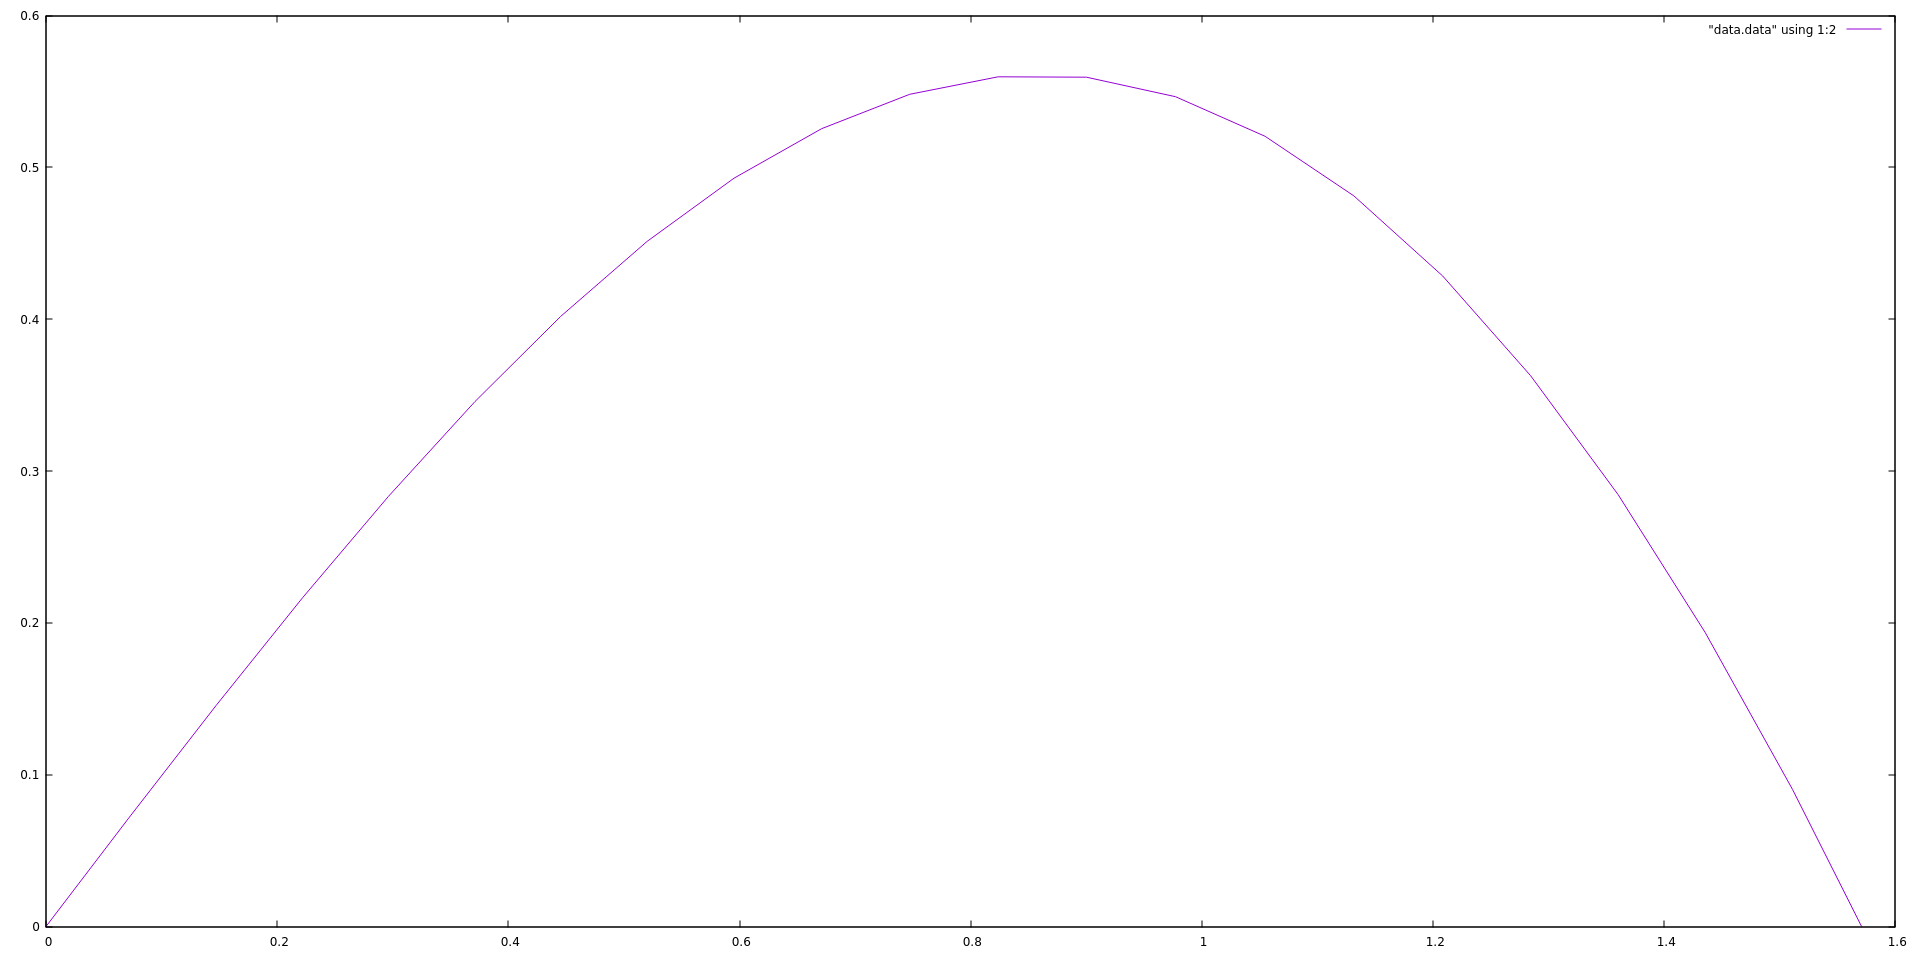
\includegraphics[width=1\linewidth]{x_1(t).png} 
\end{figure}
\newpage
\begin{figure}[h!]
$x'(t)$ $[0, \pi/2]$\\
\centering
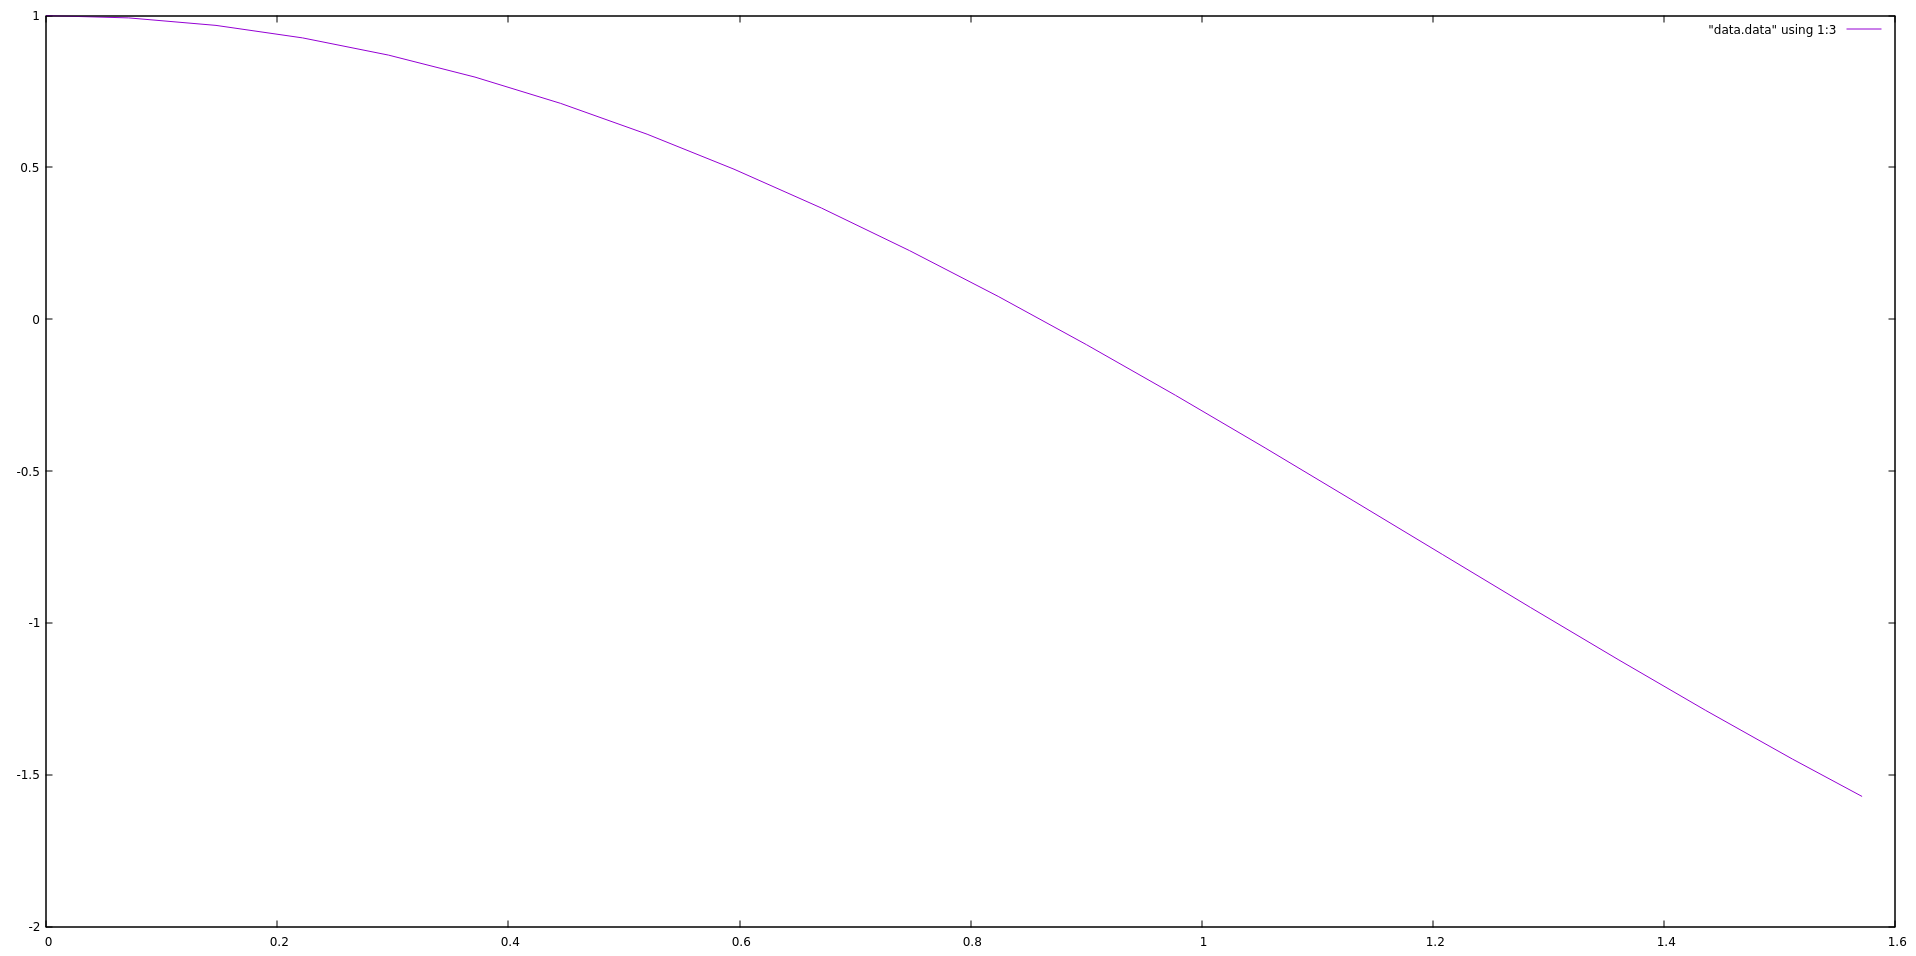
\includegraphics[width=1\linewidth]{x_2(t).png} 
\end{figure}
\begin{figure}[h!]
$p_1(t)$ $[0, \pi/2]$\\
\centering
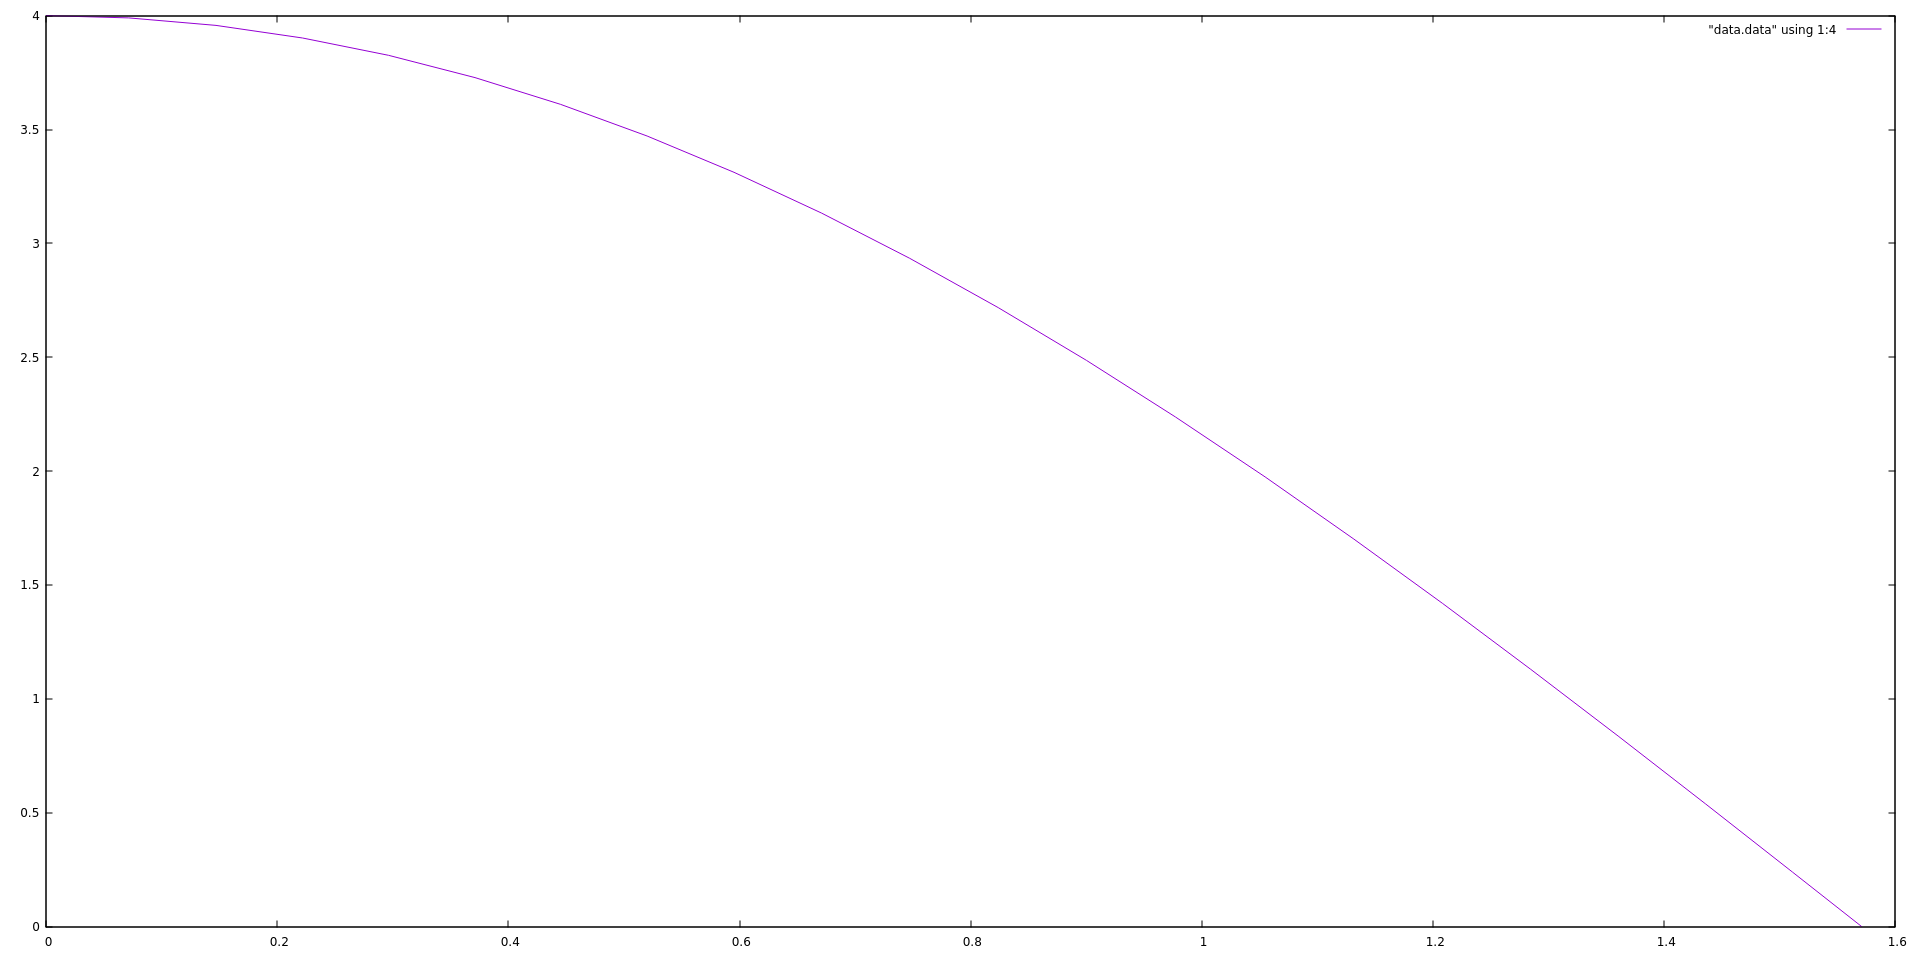
\includegraphics[width=1\linewidth]{p_1(t).png} 
\end{figure}
\begin{figure}[h!]
$p_2(t)$ $[0, \pi/2]$\\
\centering
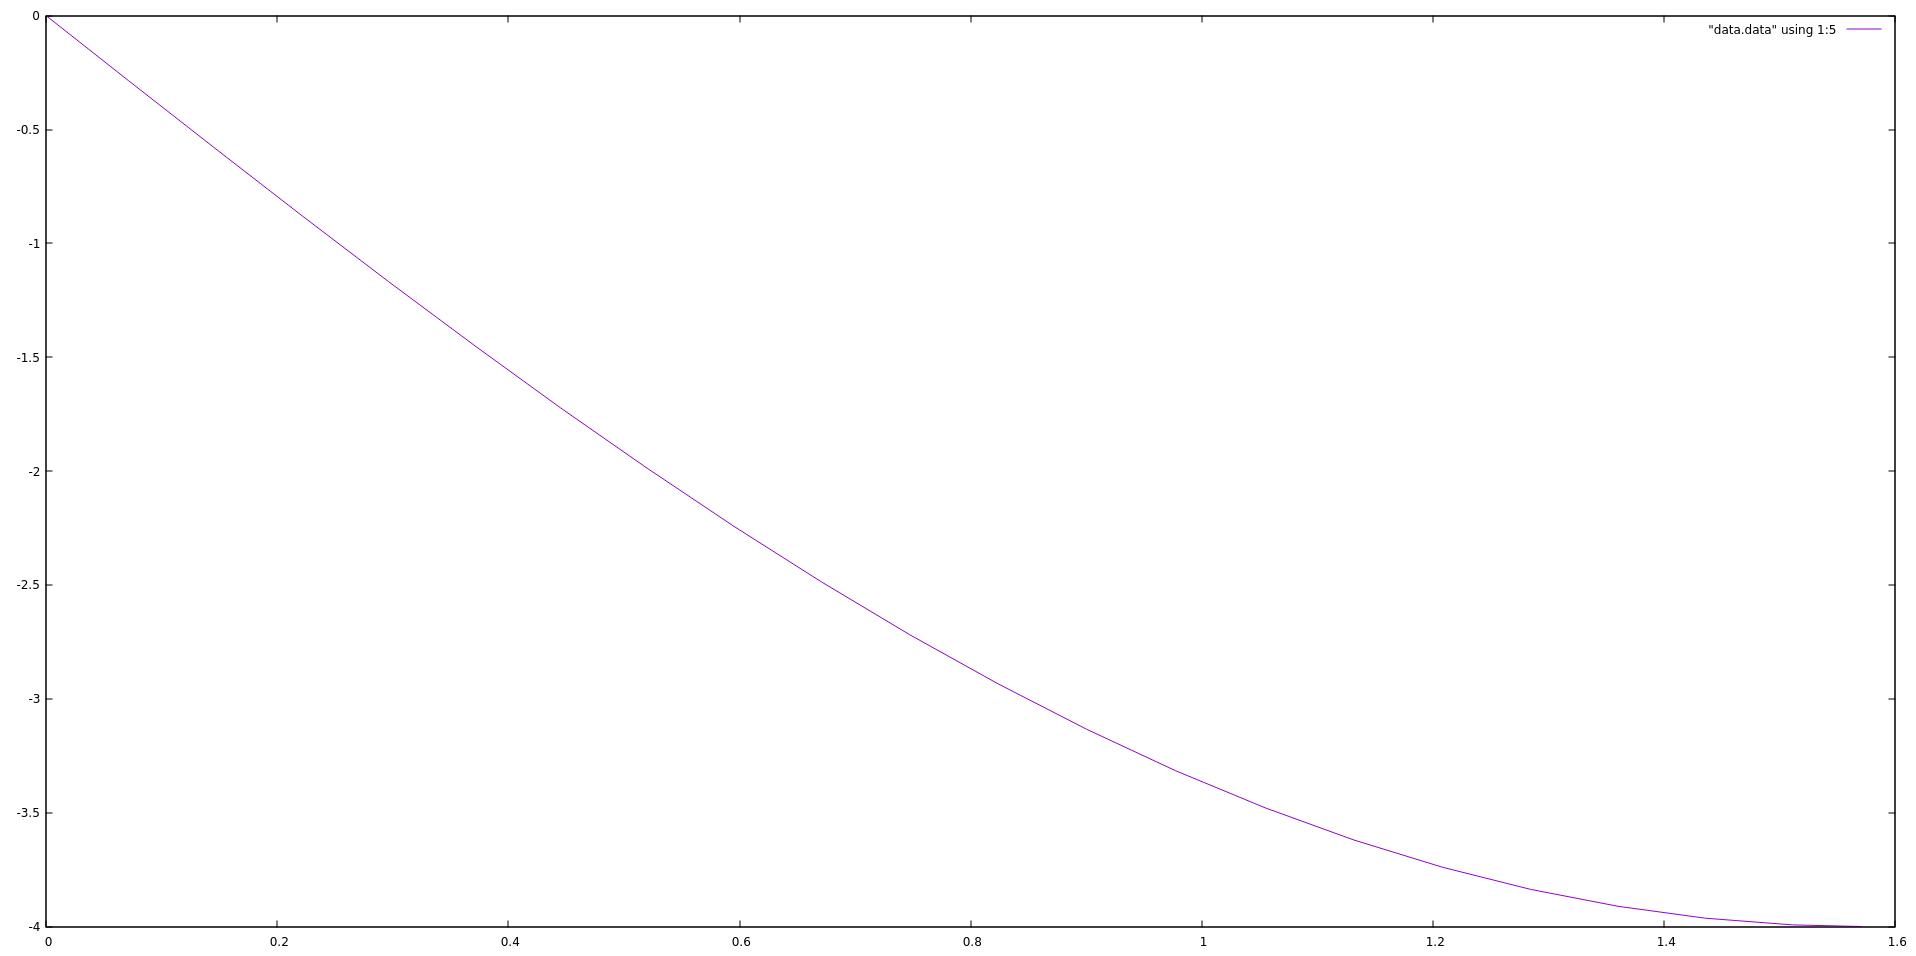
\includegraphics[width=1\linewidth]{p_2(t).png} 
\end{figure}
\begin{figure}[h!]
$integral(t)$ $[0, \pi/2]$ \\
\centering
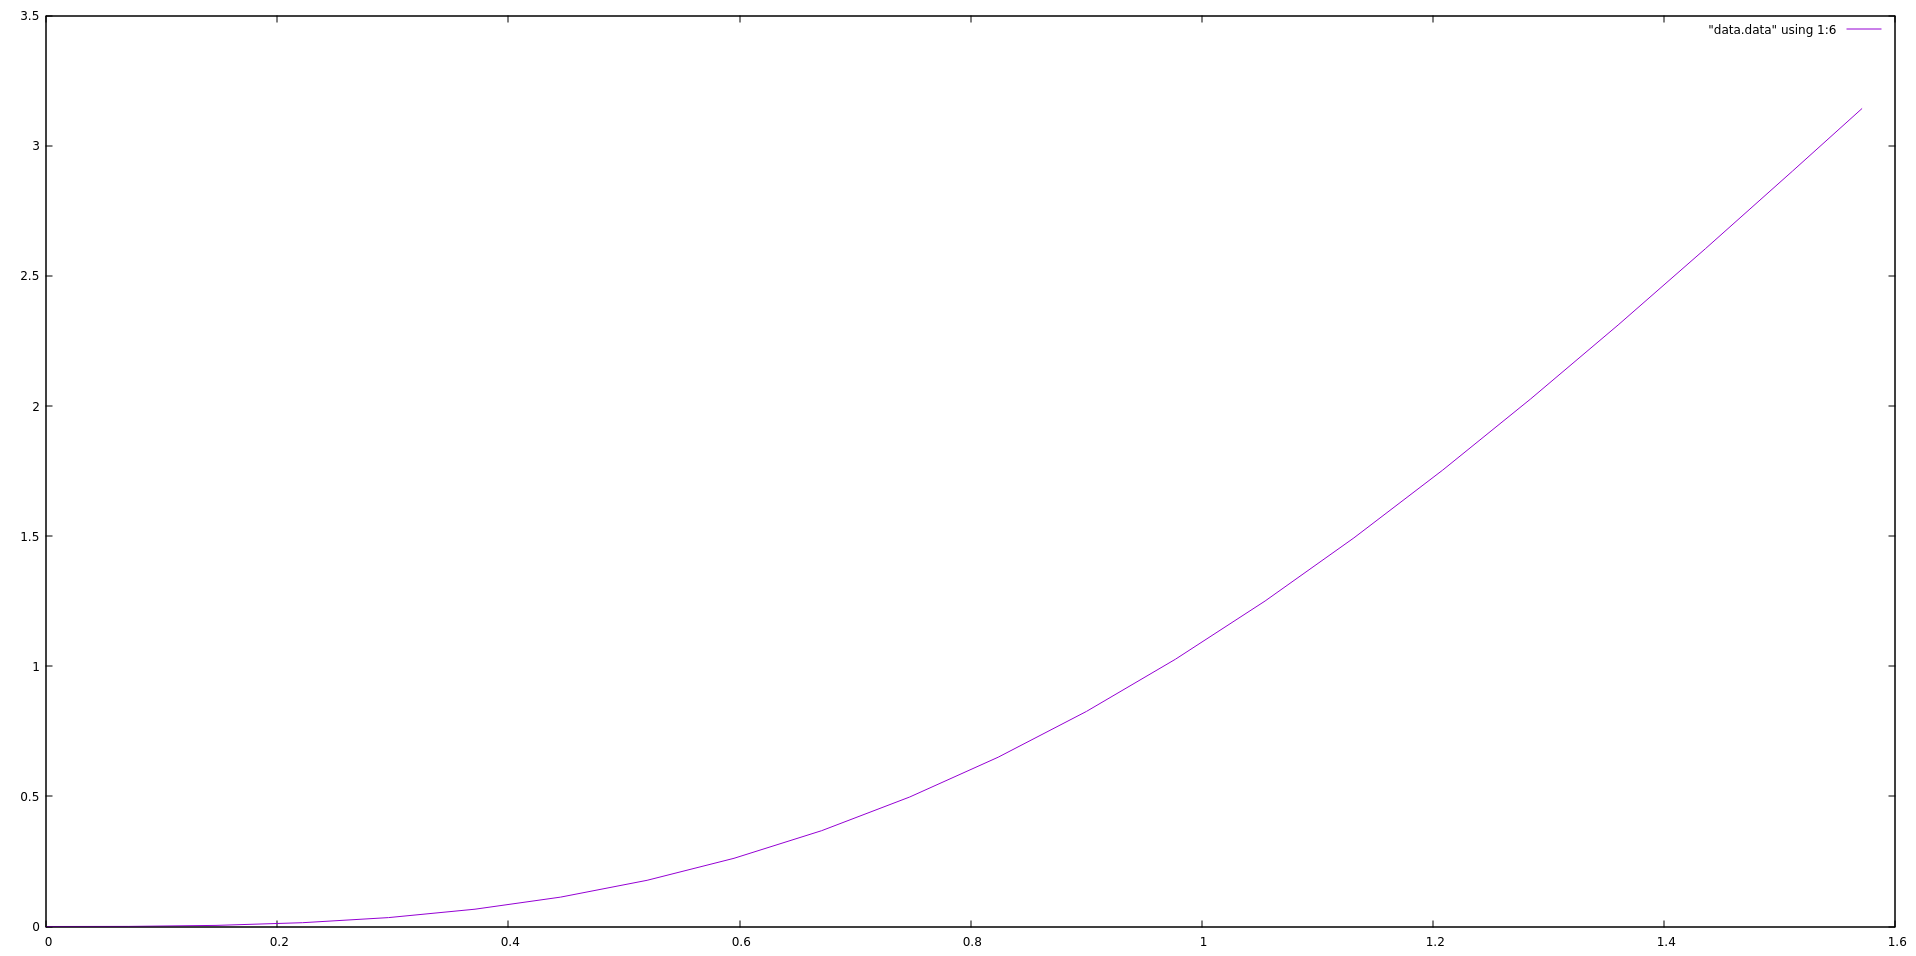
\includegraphics[width=1\linewidth]{integral(t).png} 
\end{figure}
\newpage
\textbf{Рассмотрим $\alpha = 1$}
\begin{figure}[h!]
$x_1(t)$  $[0, \pi/2]$\\
\centering
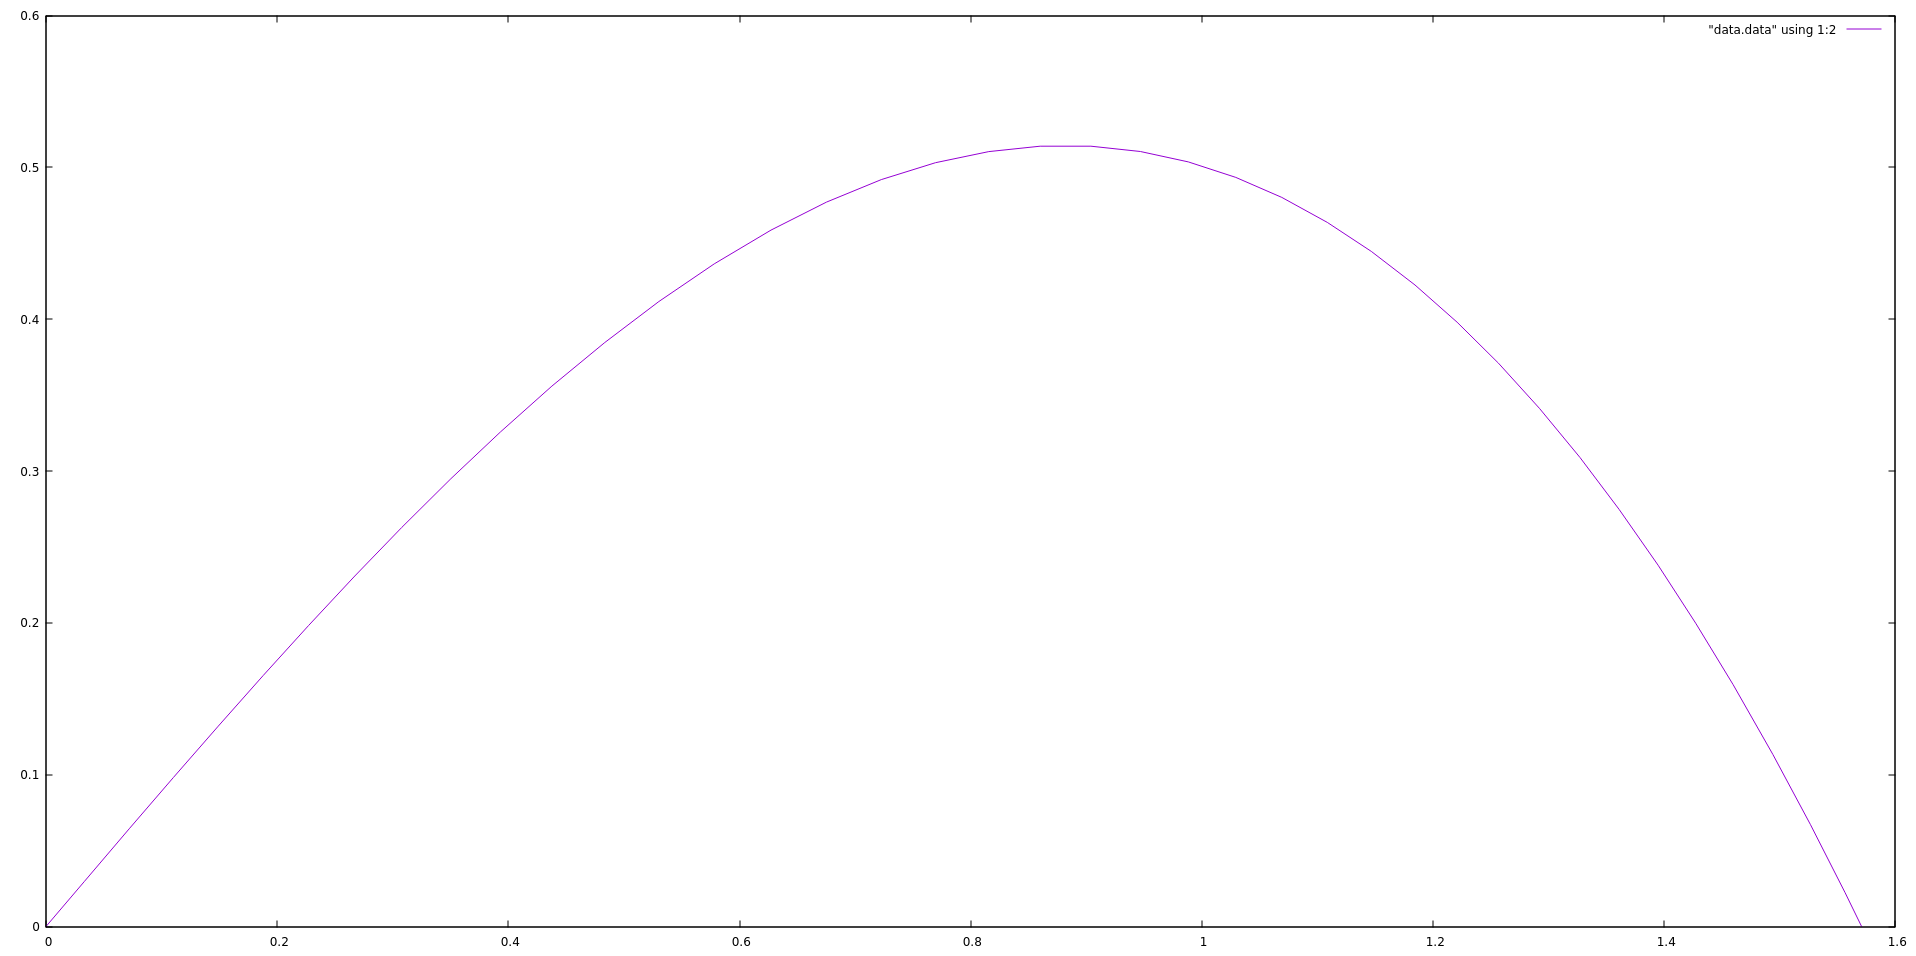
\includegraphics[width=1\linewidth]{x_11(t).png} 
\end{figure}
\newpage
\begin{figure}[h!]
$x'(t)$ $[0, \pi/2]$\\
\centering
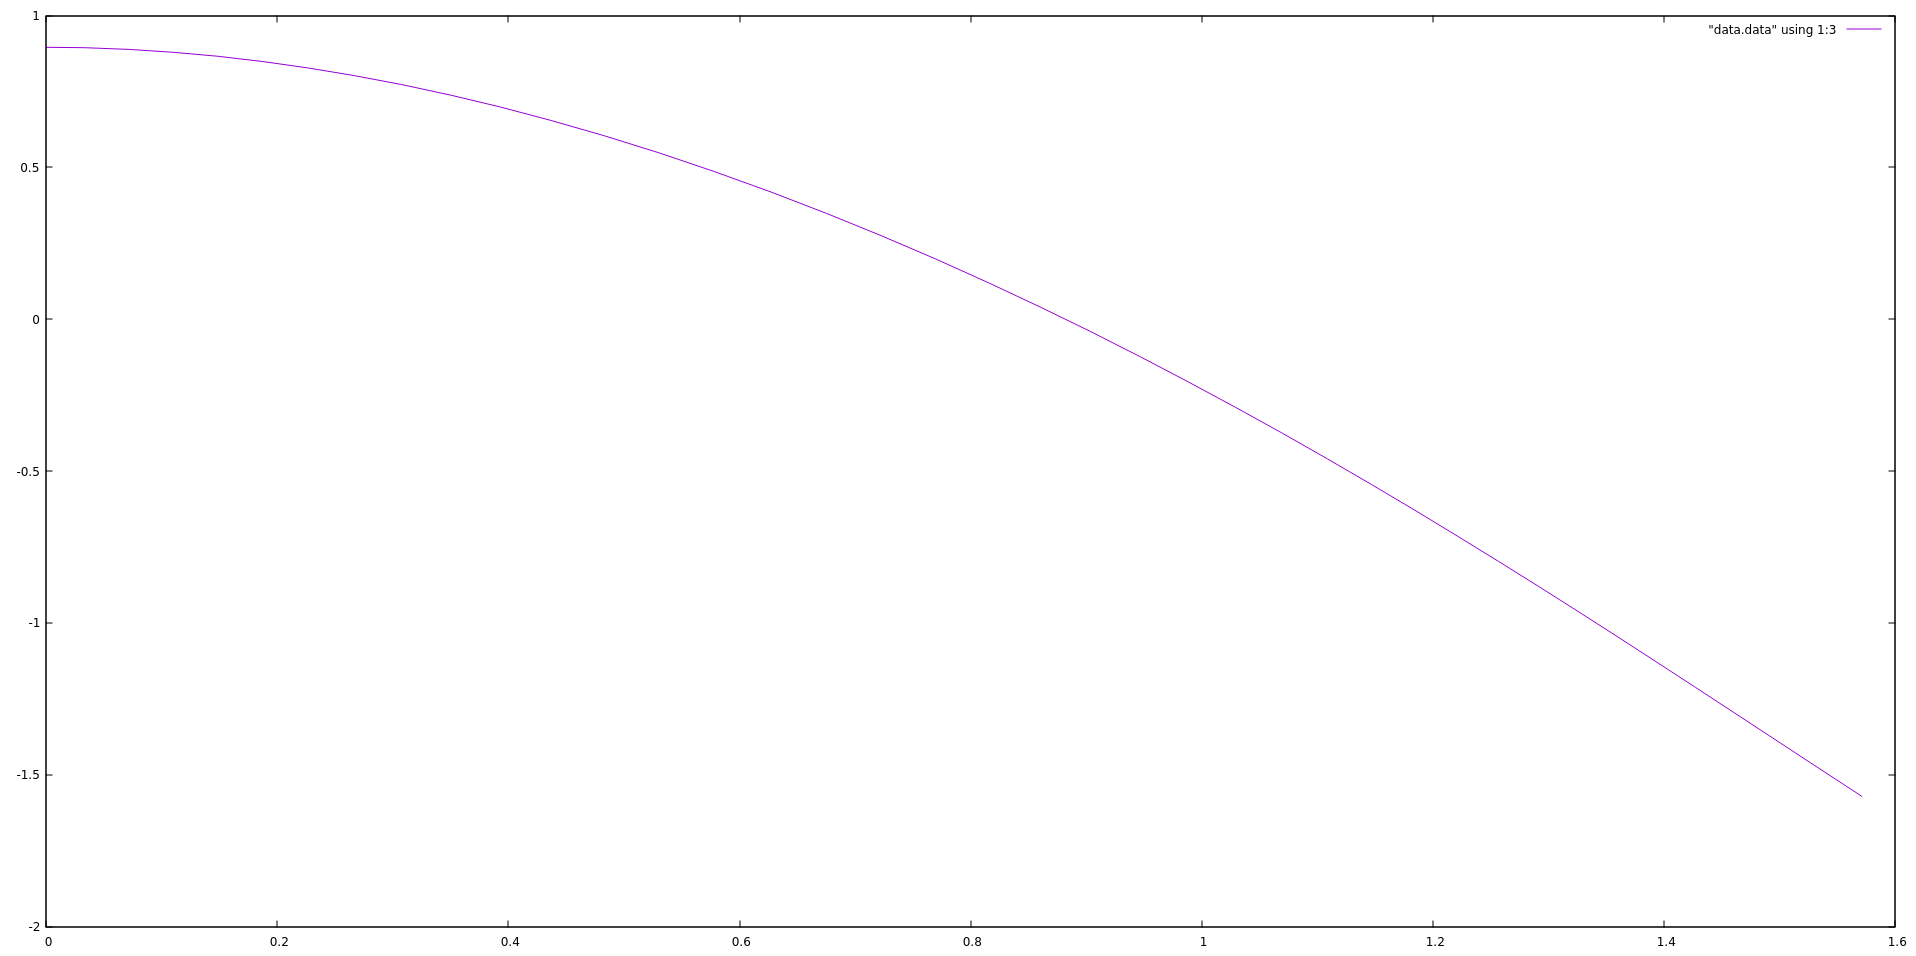
\includegraphics[width=1\linewidth]{x_21(t).png} 
\end{figure}
\begin{figure}[h!]
$p_1(t)$ $[0, \pi/2]$\\
\centering
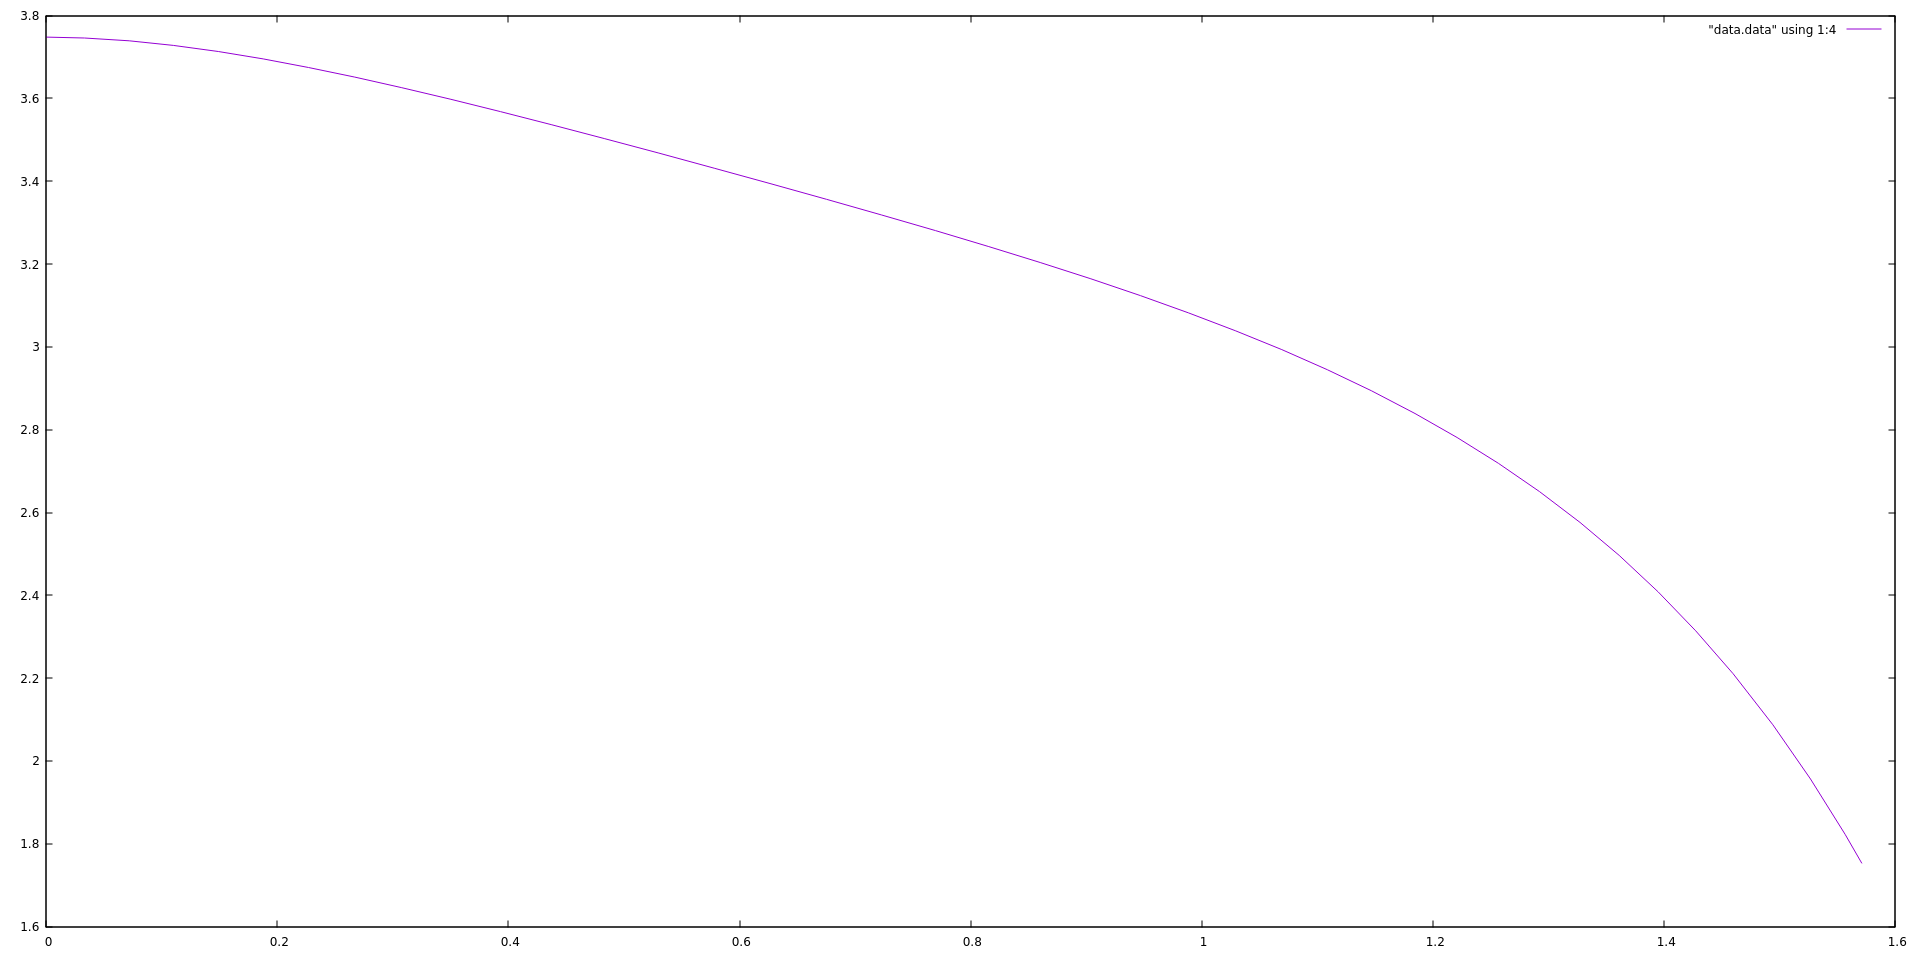
\includegraphics[width=1\linewidth]{p_11(t).png} 
\end{figure}
\begin{figure}[h!]
$p_2(t)$ $[0, \pi/2]$\\
\centering
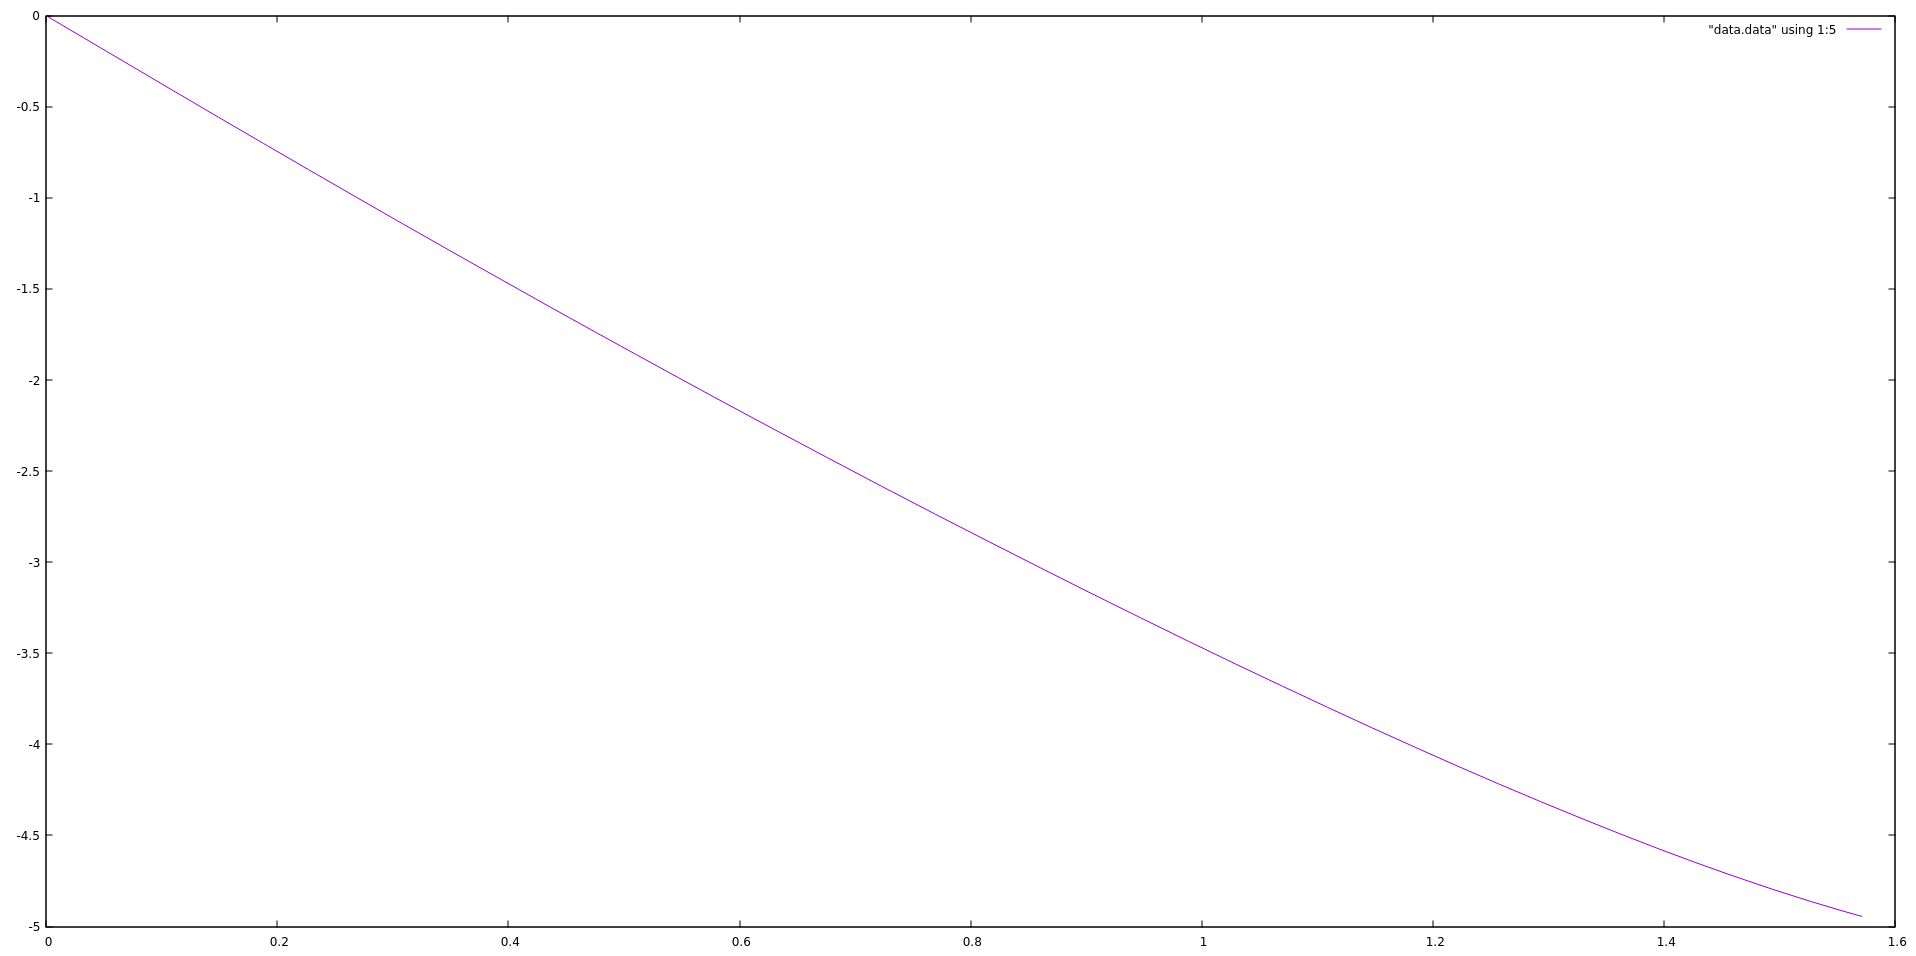
\includegraphics[width=1\linewidth]{p_21(t).png} 
\end{figure}
\begin{figure}[h!]
$integral(t)$ $[0, \pi/2]$ \\
\centering
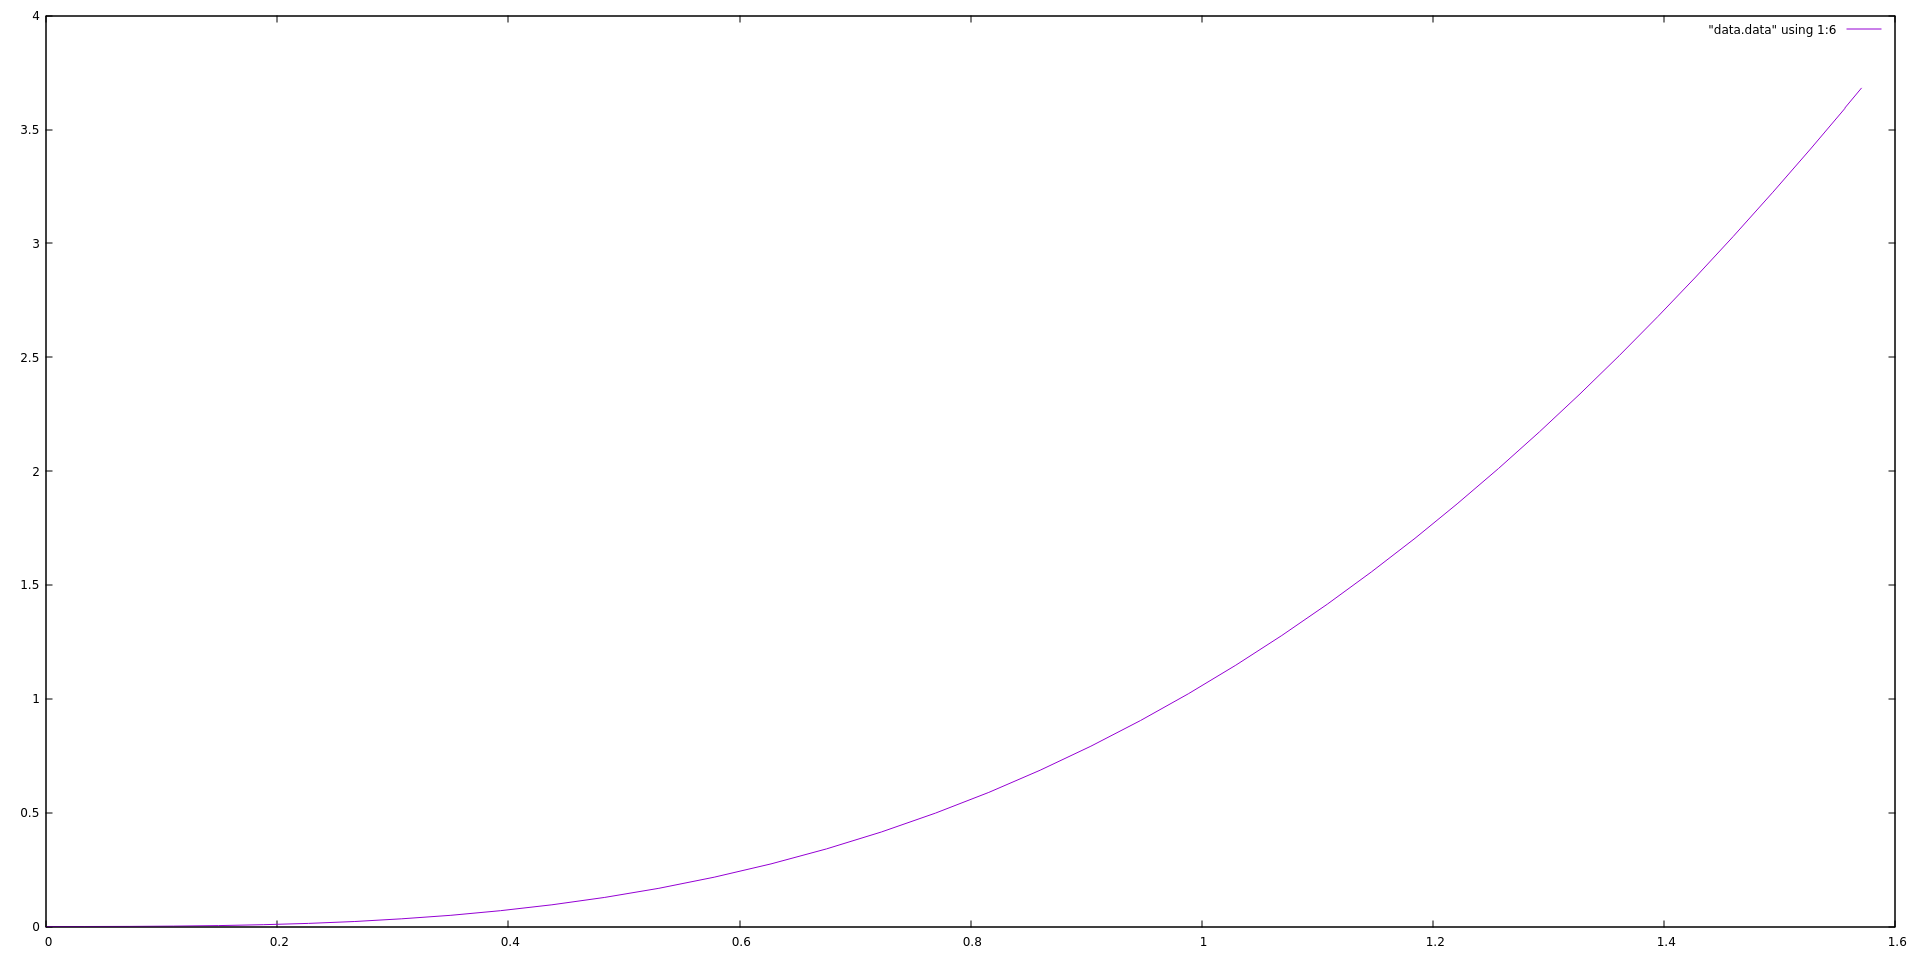
\includegraphics[width=1\linewidth]{integral1(t).png} 
\end{figure}
\newpage
\begin{figure}[h!]
Рассмотрим $\alpha = 10$ \\ $x_1(t)$  $[0, \pi/2]$\\
\centering
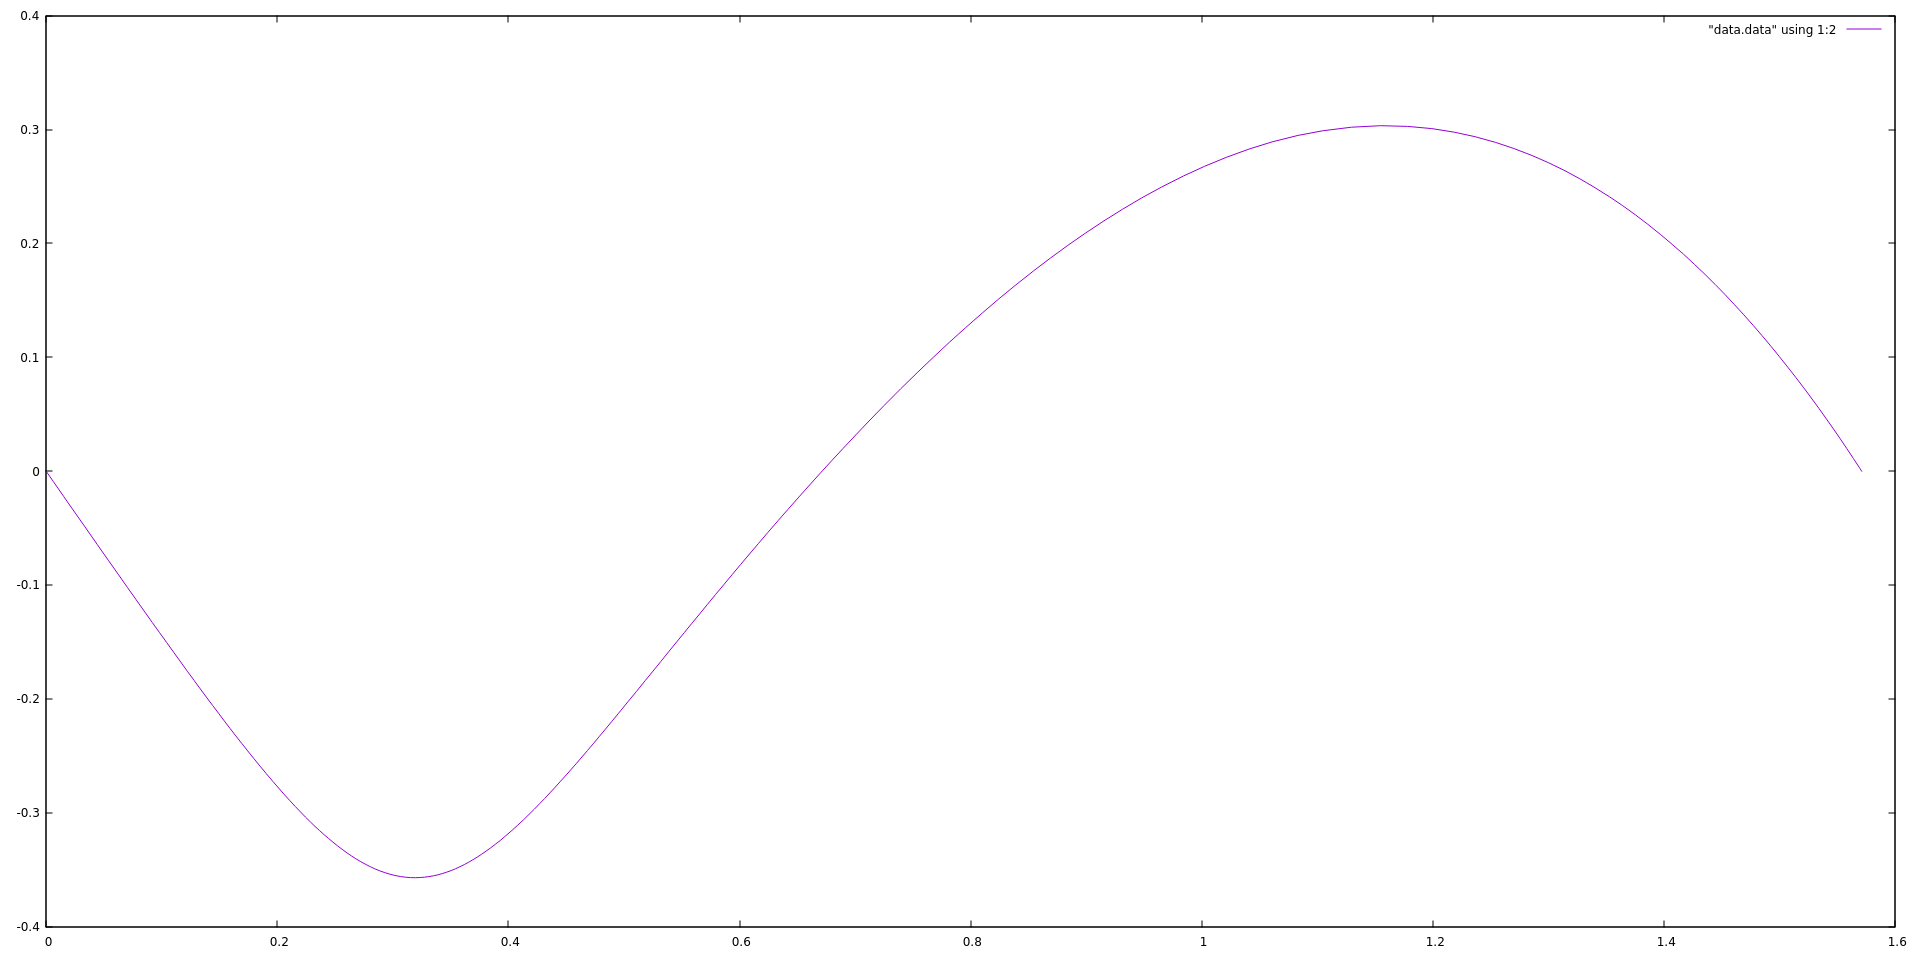
\includegraphics[width=1\linewidth]{x_110(t).png} 
\end{figure}
\newpage
\begin{figure}[h!]
$x'(t)$ $[0, \pi/2]$\\
\centering
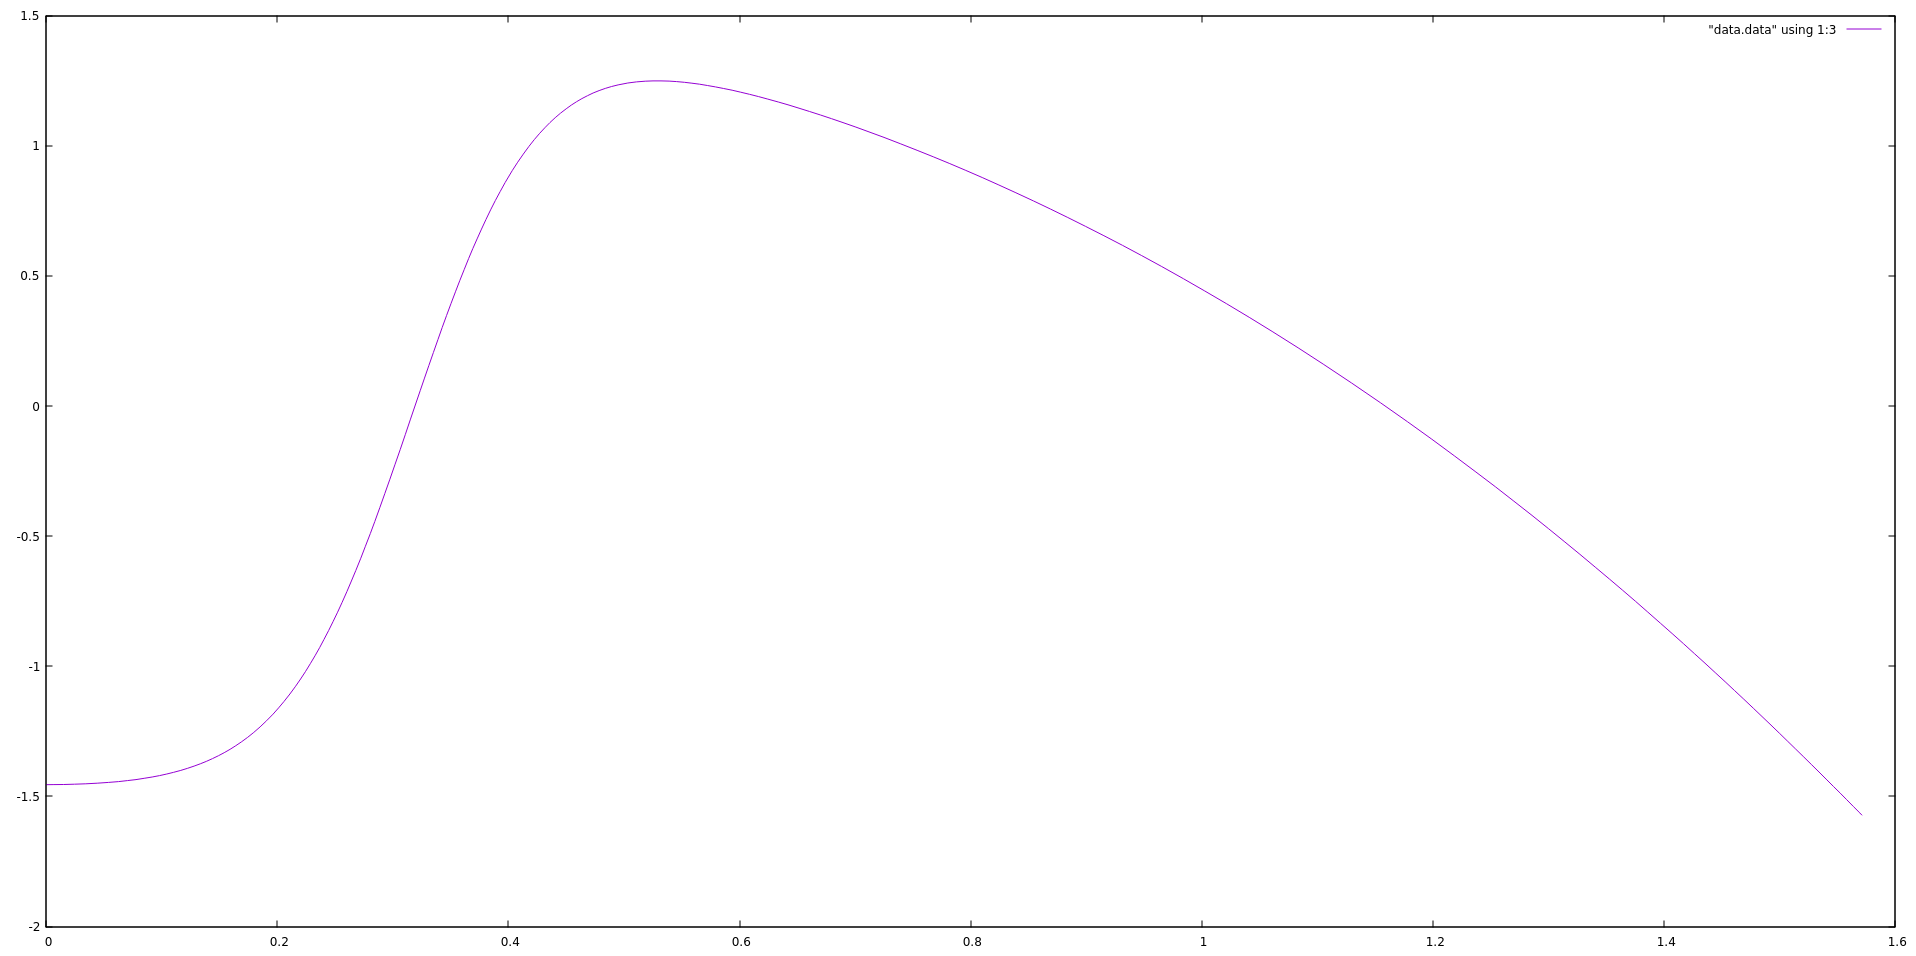
\includegraphics[width=1\linewidth]{x_210(t).png} 
\end{figure}
\begin{figure}[h!]
$p_1(t)$ $[0, \pi/2]$\\
\centering
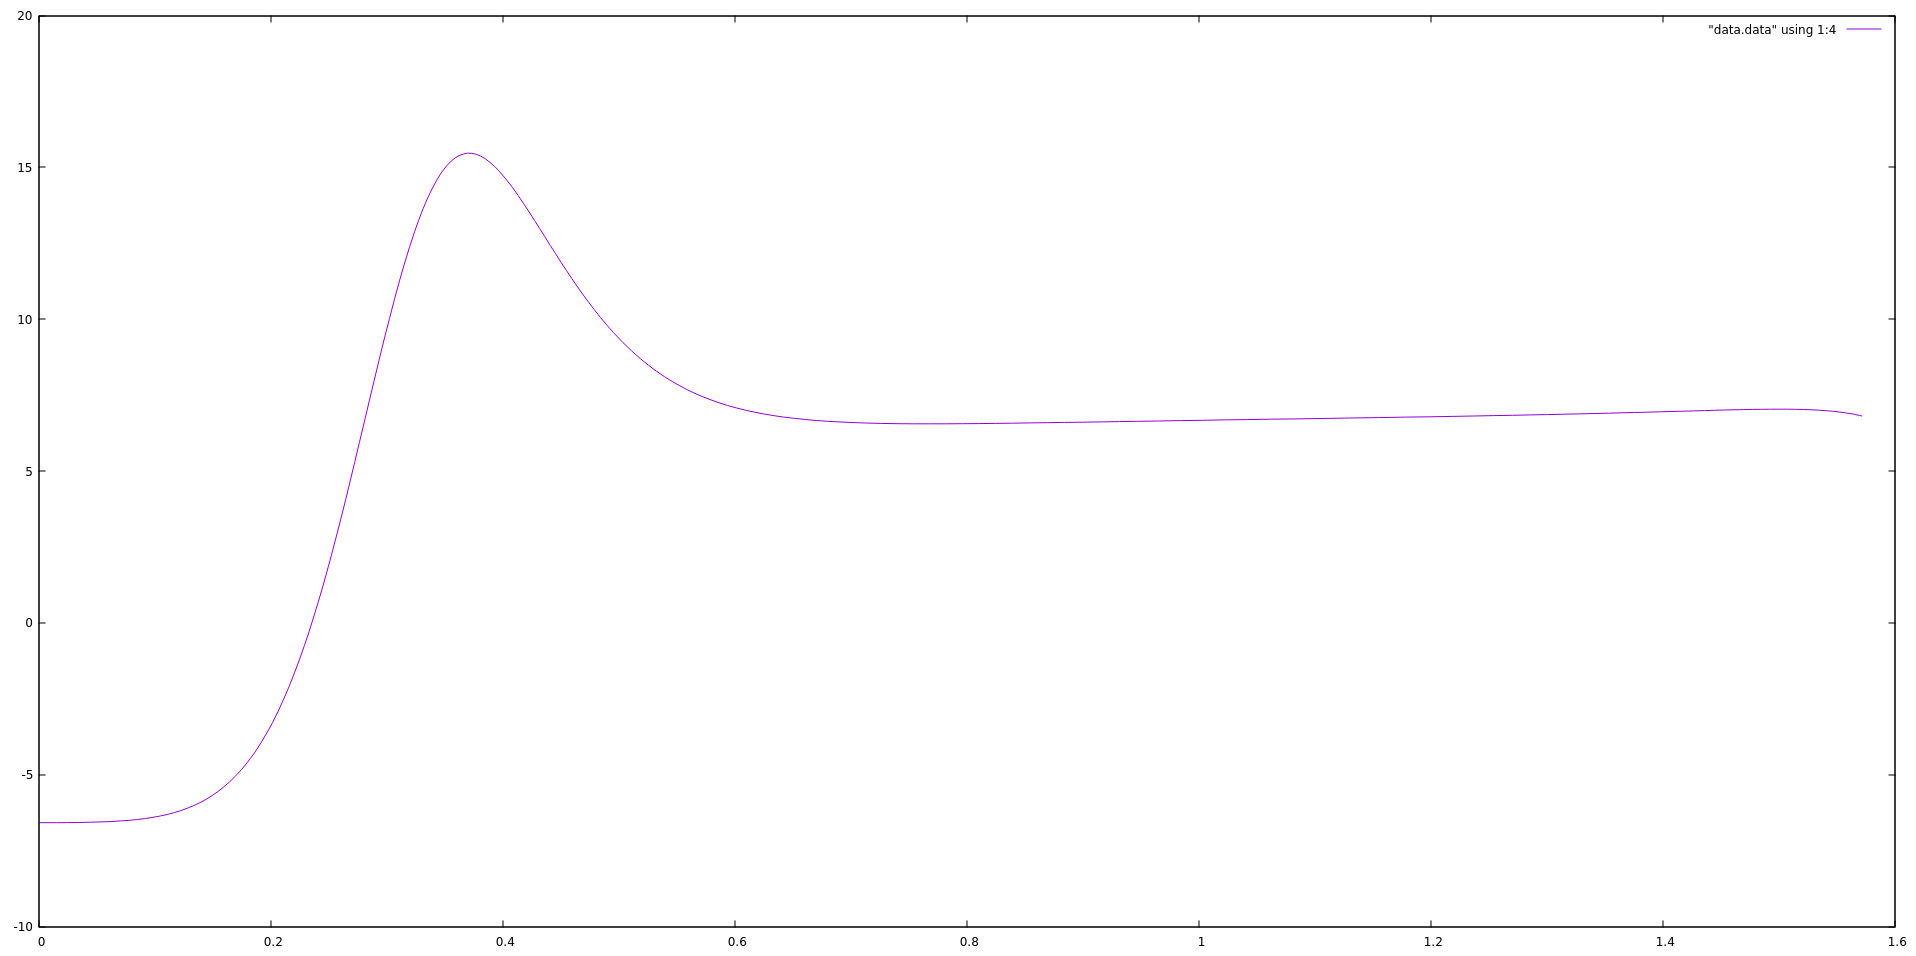
\includegraphics[width=1\linewidth]{p_110(t).png} 
\end{figure}
\begin{figure}[h!]
$p_2(t)$ $[0, \pi/2]$\\
\centering
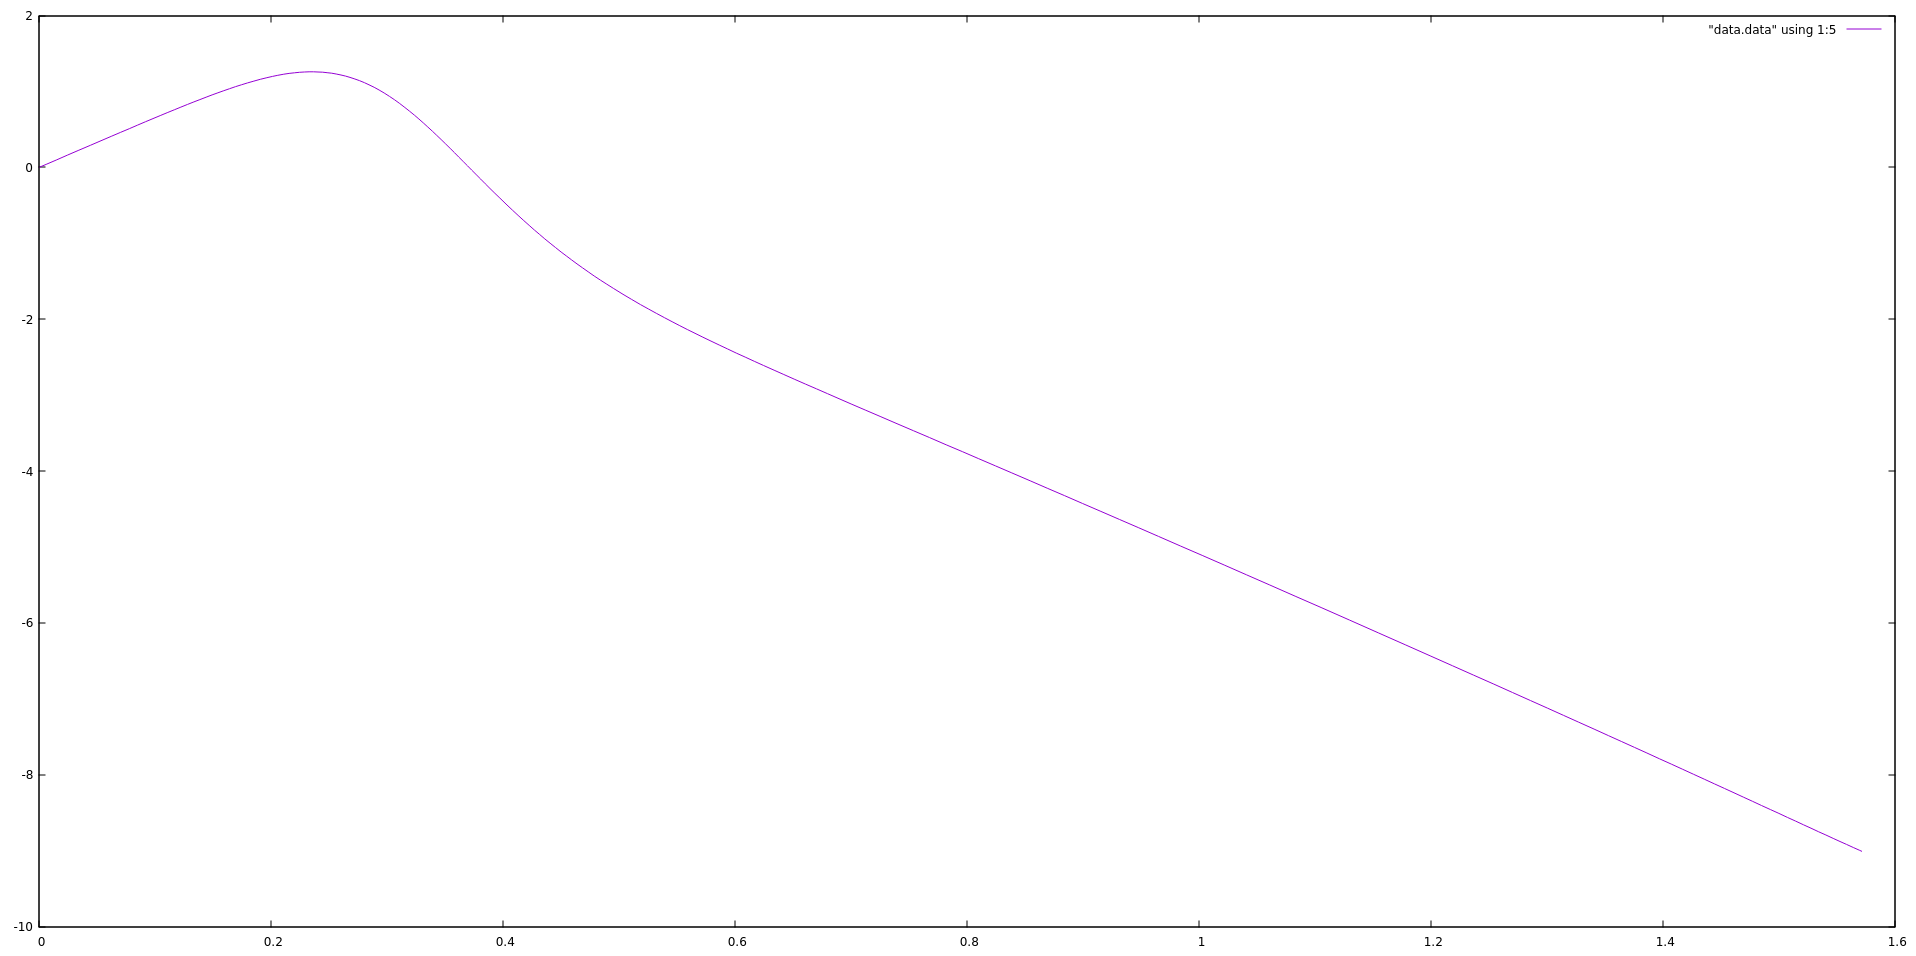
\includegraphics[width=1\linewidth]{p_210(t).png} 
\end{figure}
\begin{figure}[h!]
$integral(t)$ $[0, \pi/2]$ \\
\centering
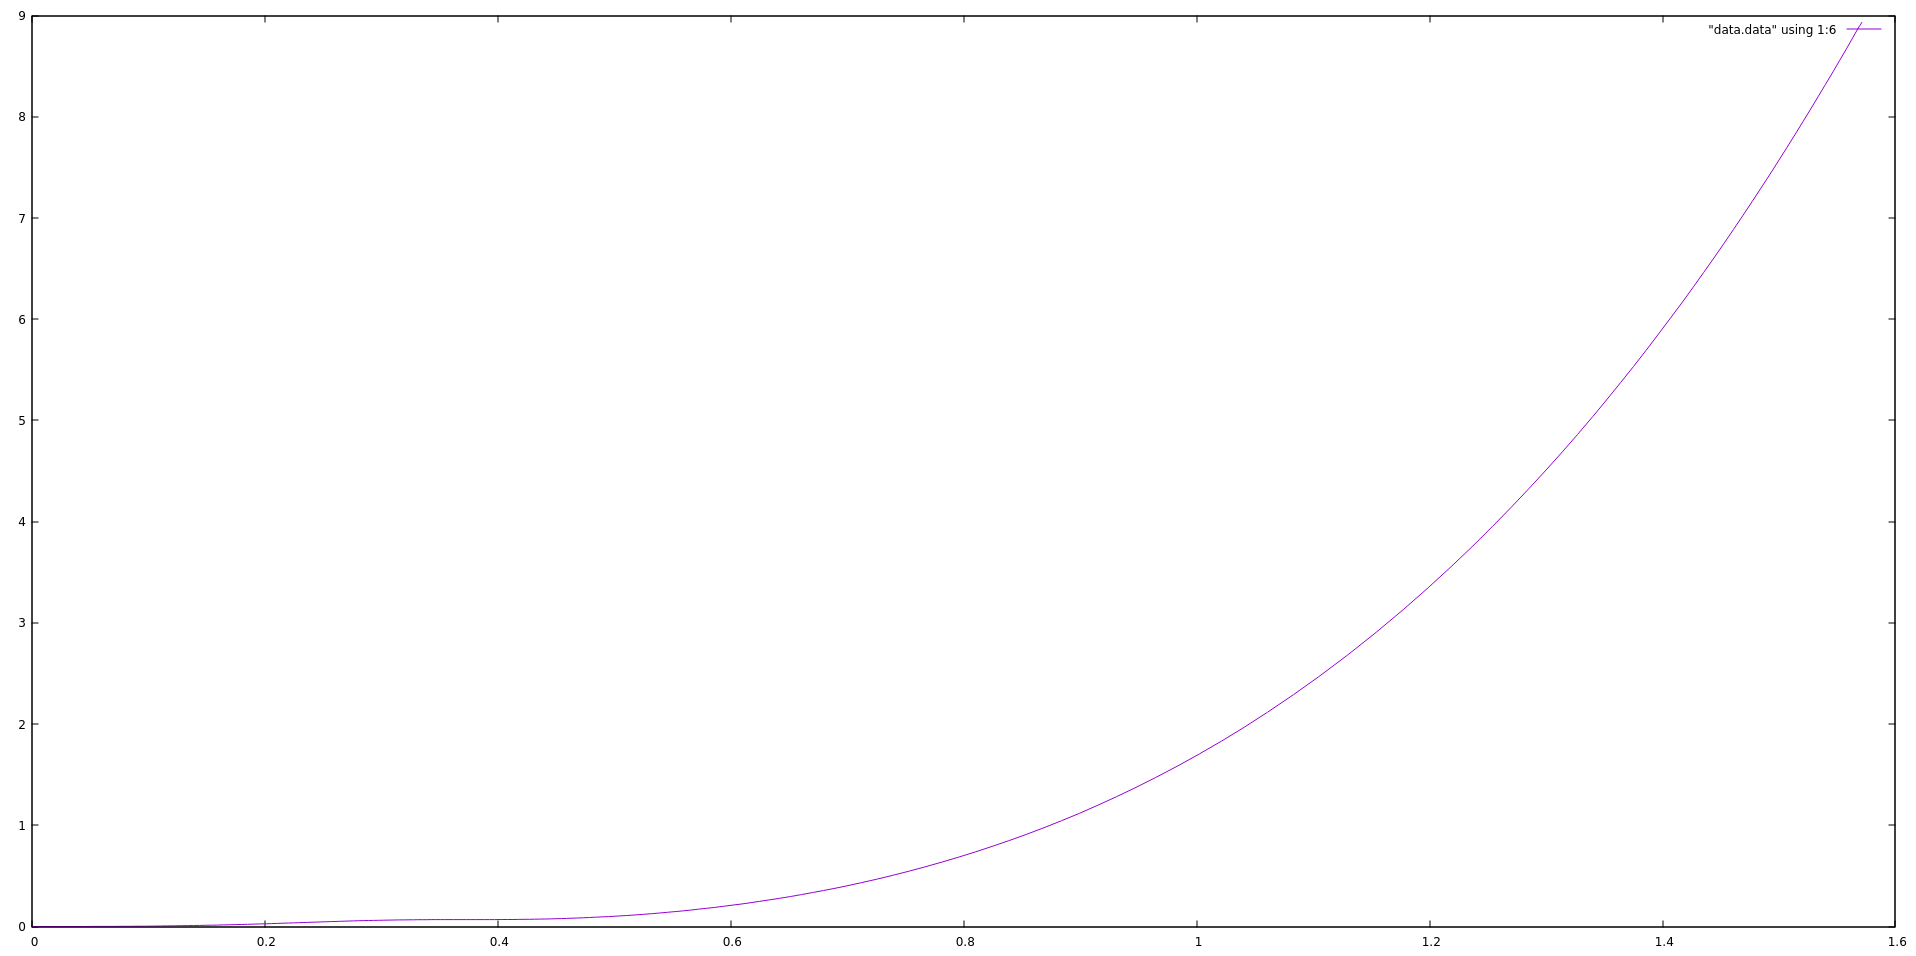
\includegraphics[width=1\linewidth]{integral10(t).png} 
\end{figure}
\end{document}
